%version of 09-25-18

\chapter{NUMBERS AND NUMERALS}
\label{ch:numbers-numerals}

Many, perhaps most, of us take for granted the brilliant notations
that have been developed for the myriad arithmetic constructs that we
use daily.  Our mathematical ancestors have bequeathed us notations
that are not only perspicuous but also convenient for computing and
for discovering and verifying new mathematical truths.  This chapter
is dedicated to sharing this legacy with the reader.

\section{Numbers}
\label{sec:numbers}

\subsection{Introduction}

Every reader will be familiar with the notion of {\it number} and with
the familiar strings, called {\it numerals}, that name numbers.
\index{numbers vs.~numerals}
\[ \approx \approx \approx \approx \approx \approx \approx \approx \approx \approx \]
Numbers and numerals embody what is certainly the most familiar
instance of a very important dichotomy that pervades our intellectual
lives: the distinction between objects and their names:

{\em Numbers are intangible, abstract objects.  Numerals are the names
  we use to refer to and manipulate numbers.}

This is a crucially important distinction!  You can ``touch'' a
numeral: break it into pieces, combine two (or more) numerals via a
large range of operations.  Numbers are intangible abstractions: you
cannot compute with them.
\[ \approx \approx \approx \approx \approx \approx \approx \approx \approx \approx \]
Historically, we have employed a broad range of mechanisms for naming
numbers.

{\ignore {\Arny I really like the idea of providing some cultural background to lure the reader.  }}
{\ignore {\Denis I also like the idea, may be we can shorten the Latin numbers
  and let some parts (examples) as an exercice...}}
{\ignore {\Arny Please propose what to omit.  I do want to point out the
  ``three levels'' of names/numerals: names that convey information
  only by cultural agreement; names that permit identification but no
  practical manipulation; {\em operational} names}}
\ignore{I am not sure, however, how much space to
  allocate.  For instance, I like the mention of Roman numerals and of
  the system that the Phoenicians used --- which I am familiar with
  mainly because of Hebrew --- but I am reluctant to go so far as to
  really discuss the formation rules of Roman numerals or the details
  of numeral formation in Hebrew and its kindred languages.}

\noindent
{\it Nicknames for ``popular'' numbers}.
%
At one extreme, we have endowed certain numbers that we are ``fond
of'' with names that do not even hint at the ``meaning of'' the named
number.  To cite just a few examples, we talk about
\begin{itemize}
\item
$\pi$: the ratio of the circumference of a circle to its diameter
\item
$e$: the base of so-called natural logarithms
\item
$\phi$: the {\it golden ratio} (one of several word-names for $\phi$)
  that can be observed in nature, e.g., in the leaf patterns of plants
  such as pineapples and cauliflower
{\ignore  {\Denis we will develop some Maths involving $\phi$  in the chapter
    recurrences and Fibonacci numbers...}}
{\ignore {\Arny That is great!!  I just added a mention of that below!}}
\item
Avogadro's number: a fundamental quantity discussed in chemistry and
physics.  We include this number-name to indicate that not all
special numbers' nicknames are single letters.
\end{itemize}
Nickname-based numerals give no information about the named number:
they do not help anyone (except possibly the {\it cognoscenti:} the
``in-crowd'') {\em identify} the named number, and they do not help
anyone manipulate---e.g., compute with---the named number.  These
names are valuable only for {\em cultural} purposes, not mathematical
ones.

We want to be totally clear about our intended message.  It is the
{\em names} of the numbers we have entioned that convey no operational
information.  Regarding the numbers themselves, each is attached to
valuable science and/or mathematics!  We shall expose some of this
mathematics as we discuss $e$ in the current chapter, as we revisit
$\pi$ and $e$ in Chapter~\ref{ch:Summation}, and as we revisit $\phi$
in Chapter~\ref{ch:Recurrences}.

\medskip

\noindent
{\it Alphabet-based systems.}
%
Several cultures have developed systems for naming arbitrary integers
by using their alphabets in some manner.

One such system that is still visible in European cultures within
constrained contexts comprises so-called {\it Roman numerals}.  One
stills observes these, for instance, as the hour markers on the faces
of ``classical'' clocks and as timestamps on the cornerstones of
official buildings.  Roman numerals are formed from a constrained set
of letters from the Latin alphabet:

\begin{tabular}{c|c}
{\it Letter} & {\it Numerical value} \\
\hline
I  & 1 \\
V  & 5 \\
X  & 10 \\
L  & 50 \\
C  & 100 \\
D  & 500 \\
M  & 1000
\end{tabular}

\noindent
The formation rules for Roman numerals of length exceeding $2$ are a
bit complicated, but {\em roughly}, a letter to the right of a higher
valued letter augments the value of the numeral (e.g., DCL $=650$, XVI
$=16$), while a letter to the left of a higher valued letter lowers
the value (e.g., MCM $=1900$, XLIV $=44$).

Yet another way to craft numerals from letters is observable in
systems such as is used with the Hebrew alphabet, which incorporates
ideas used by the ancient Egyptians, Phoenicians, and Greeks.  Hebrew
assigns the following respective values to the $22$ letters of its
alphabet.
\[ 1, 2, 3, 4, 5, 6, 7, 8, 9, 10,
20, 30, 40, 50, 60, 70, 80, 90, 100,
 200, 300, 400
\]
Numerals are then formed as strings of single occurrences of letters,
by accumulating the letters' numerical values.  Numbers that are too
large to be named using ``words'' comprising single letter-instances
often allow repeated letter instances or using auxiliary words, in a
mixed-mode manner similar to our writing the number $5000$ as ``$5$
thousand''.
{\ignore {\Denis I am not familiar with Hebrew, I would like to know how to
  address the unicity of the writing numbers...}}
{\ignore {\Arny I am familiar with Hebrew numerals in only two contexts:

(a) They are used widely with the (Hebrew) calendar.  The names of the
  Hebrew months are Babylonian in origin.  The days are always
  denoted by Hebraic numerals.  Within a religious framework, there is
  a number that is associated with the age of the world (since
  ``creation'').  This number was computed by a Catholic monk many
  centuries ago, based on his reading of the Old Testament.  The Jews
  have adopted this number --- and they usually express it with a
  ``mixed'' Hebraic numeral of the form ``5 thousands plus abcd''.  In
  a semi-religious context such as a gravestone, e.g., all of the
  relevant numerals are denoted by Hebraic numerals.

(b) They are used widely as part of a semi-mystical exercise called
  ``gematria''.  Since every numeral is potentially a word, certain
  numbers gain semi-mystical importance.  The mystics use this a lot
  in interpreting biblical texts.  Perhaps the most POPULAR instance
  of gematria relates to the Hebrew word for ``life'': this two-letter
  word is ``chai''.  It has the numerical value 18.  Even nonreligious
  Jews will acknowledge this by, e.g., giving gifts that are integer
  multiples of 18.  For instance, a gift in the amount of 50 dollars is
  usually ``rounded up'' to 54.

I BELIEVE that the numerals were once used more widely, but I know
little about that.}}

Alphabet-based systems for creating numerals are more useful than
nickname-based systems in that they {\em do} allow anyone to {\em
identify} any named number. Indeed, one can (algorithmically)
convert any Roman numeral or any Hebrew numeral to a decimal numeral
for the same number.  However, any reader who is familiar with
alphabet-based systems will recognize a major drawback of such
systems: It is {\em exceedingly difficult} to do any but the most
trivial arithmetic using such systems' numerals.  Two simple examples
using Roman numerals will make our case:
\begin{itemize}
\item
Square CC.  This is, of course, trivial using our familiar decimal
numerals: an elementary school student can compute $200 \times 200 \ =
\ 40,000$.  But even in an early course on programming, one would not
assign the general ``multiply numbers using Roman numerals'' problem
as a first assignment.

\item
Substract MCMXCVIII from MMII.  We all know, of course, that the answer
is IV, but determining this is usually done by converting to decimal numerals
($2002-1998$).
\end{itemize}

\noindent
{\it Positional number systems.}
%
In our daily commerce, we typically deal with numerals that are formed
within a {\it base-$b$ positional number system,}
\index{numerals in a (base-$b$) positional number system}
%
i.e., by strings of {\it digits} from a set of the form $\{0, 1, 2,
\ldots, \overline{b-1}\}$, often embellished with other symbols, such as
a {\em radix point},\footnote{The use of a period as the radix point
  is a US convention; in much of Europe, a comma usually denotes the
  radix point.}~and sometimes a leading ``$+$'' or ``$-$'' to
indicate, respectively, the denoted number's positivity or negativity.
\[ \approx \approx \approx \approx \approx \approx \approx \approx \approx \approx \]
{\em We employ the notation ``$\overline{b-1}$'' to remind ourselves
  that in this context ``$b-1$'' is a digit, not a string; for
  instance, when $b = 10$ (the common {\em decimal} base),
  $\overline{b-1}$ is the digit $9$.  }
\[ \approx \approx \approx \approx \approx \approx \approx \approx \approx \approx \]
We discuss positional number systems in detail in
Section~\ref{sec:Numerals}.  For now, we settle for a few examples:
\begin{itemize}
\item
Most of our daily work employs the base-$10$ ({\it decimal}) system,
whose digits comprise the set $\{0, 1, 2, 3, 4, 5., 6, 7, 8, 9\}$; the
system's radix point is usually called a {\em decimal point}.

\item
Because electrical and electronic circuitry are (for the most part)
built using {\it bistable} devices---e.g., switches that are either
{\em on} or {\em off}---the system most often employed when dealing
with such circuitry and its end products (say, computers) is the
base-$2$ ({\it binary}) system, whose digits---usually called {\it
  bits}---comprise the set $\{0, 1\}$.

\item
Because of its small repertoire of digits, the binary system's
numerals are quite long---roughly $3$ times longer than decimal
numerals.  For instance,
\[ 32,768 \ \mbox{ base $10$} \ \ = \ 1,000,000,000,000,000 \ \mbox{
  base $2$}
\]
In order to make these numerals easier for humans to deal with, small
sequences of bits are often aggregated to form larger number bases---but
still powers of $2$.  Two aggregations have been particularly popular:
  \begin{itemize}
  \item
By aggregating length-$3$ sequences of bits, one converts binary
numerals to base-$8$ ({\it octal}) numerals; the octal digits comprise
the set $\{0, 1, 2, 3, 4, 5, 6, 7\}$.
  \item
By aggregating length-$4$ sequences of bits, one converts binary
numerals to base-$16$ ({\it hexadecimal}) numerals; the hexadecimal
digits comprise the set
\[ \{0, 1, 2, 3, 4, 5, 6, 7, 8, 9, \overline{10}, \overline{11},
\overline{12}, \overline{13}, \overline{14}, \overline{15}\}.
\]
{\it Note:} We have written the hexadecimal digits in decimal, to make
them easy to read, but we have placed overlines above the $2$-digit
(decimal) numerals ``$10$'', ``$11$'', ``$12$'', ``$13$'', ``$14$'',
and ``$15$'' as a reminder that each represents a single hexadecimal
digit, not a $2$-digit numeral.
  \end{itemize}
\end{itemize}


\subsection{A Brief Biography of Our Number System}
\label{sec:number-taxonomy}
\index{number system!biography}

We begin our study of arithmetic with a short taxonomy of {\it
  numbers}, the objects that arithmetic was invented to explicate and
exploit.  Although we assume that the reader is familiar with the most
common classes of numbers, we do spend some time highlighting
important features of each class, partly, at least, in the hope of
heightening the reader's interest in this most basic object of
mathematical discourse.

We present the four most common classes of numbers in what is almost
certainly the chronological order of their discovery/invention.
\[ \approx \approx \approx \approx \approx \approx \approx \approx \approx \approx \]
{\em Did humans {\em invent} these classes of numbers to fill specific
  needs, or did we just {\em discover} their pre-existing selves as
  needs prompted us to search for them?  The great German
  mathematician Leopold Kronecker,
\index{Kronecker, Leopold}
as cited in \cite{Bell86} (page 477), shared his viewpoint on this
question:} ``God made the integers; all else is the work of man.''
\[ \approx \approx \approx \approx \approx \approx \approx \approx \approx \approx \]
A pleasing narrative can be fabricated to account for our multi-class
system of numbers.  In the beginning, the story goes, we needed to
count things (sheep, bottles of oil, weapons, \ldots), and the
positive {\it integers}\index{number!integer} were discovered to serve
this need.  As accounting practices matured, we needed to augment this
class with the number zero \index{number!zero ($0$)} ($0$), to allow
merchant $A$ to keep track of the inventory remaining after the last
flask of wine is sold, and with the negative integers,
\index{number!negative} to allow the merchant's banker to record $A$'s
credit balance after taking a loan.  
{\ignore {\Denis right, nicely said, but the zero wasn't mainly created for the
sake of computing idle positions in additions?} } 
{\ignore {\Arny I was aiming
for a history of NUMBERS, not numerals.  There is no numeral for 0
in Latin or Hebrew, but there were certainly word-names for zero.  I
believe that the numeral is not needed until you have a positional
number system.}}
The class of integers was now complete, even though a variety of
special classes of integers that warranted special attention for
reasons ranging from the religious to the intellectual remained to be
discovered.  As society matured, humans began to share materials that
had to be subdivided---cloth, grain, etc.---rather than partitioned in
discrete units.  We needed to invent the {\it rational numbers}
\index{number!rational}
%
to deal with such materials.  Happily for the mathematically inclined,
the rational numbers could be developed in a way that allowed one to
view an integer as a special type of rational.  This meant that our
ancestors could build upon the systems they had developed to deal with
integers, rather than scrapping those systems and starting anew.
\[ \approx \approx \approx \approx \approx \approx \approx \approx \approx \approx \]
{\em This quest for {\em extendible} frameworks rather than isolated
  unrelated frameworks is a hallmark of mathematical thinking.}
\[ \approx \approx \approx \approx \approx \approx \approx \approx \approx \approx \]
We now enter the realm of ``semi-recorded'' history in the West: the
Babylonians, the Egyptians, the Greeks, and others.  ``Practical''
mathematics was invented---and reinvented---to accommodate pursuits as
varied as astronomy and architecture.  Our mathematical stalwarts, the
integers and the rationals, did not seem to be able to deal with all
of the measurements that we wanted to make, calculations that we
wanted to do, structures that we wanted to design.  So, we
approximated and ``fudged'' and got pretty much where we wanted to
get.  The standard story at this point (at least in the West) is that
the ancient Greeks began to try to systematize mathematical knowledge
and practice.  The Greek mathematician and geometer Euclid
\index{Euclid} and members of his school verified---via one of the
first {\em proofs} in recorded history---the uncomfortable fact that
the lengths of portions of eminently buildable structures were not
``measurable,'' by which they meant {\em not rational}.  The poster
child for this phenomenon was the hypotenuse of the isosceles right
triangle $T$ with unit-length legs.  Thanks to the well-known theorem
of the Greek mathematician Pythagoras \index{Pythagoras} even
schoolchildren nowadays know that the length of this eminently
buildable line is $\sqrt{2}$.  What Euclid discovered---and what is
likely not known by {\em all} schoolchildren---is: {\em There
  is---provably!---no way to find integers $p$ and $q$ whose ratio is
  $\sqrt{2}$, the length of $T$'s hypotenuse.}\footnote{We present a
  version of Euclid's proof in Proposition~\ref{thm:sqrt(2)}.}
\[ \approx \approx \approx \approx \approx \approx \approx \approx \approx \approx \]
It is worthwhile digressing here with some supplementary material so
that you do not have to take our word for the mathematical facts
underlying our story.

Even though the so-called {\it Pythagorean Theorem} is widely known,
at least informally, it is worthwhile to provide a formal statement of
this seminal result.  Quite aside from reviewing the Theorem's
important content, this statement will provide the reader one more
opportunity to ponder the ``music'' of mathematical discourse.

Let us be given a triangle $T$ with vertices $A$, $B$, and $C$.  Use
the lefthand grey triangle in Fig.~\ref{fig:unitsquare} as a model.
\begin{figure}[htb]
\begin{center}
       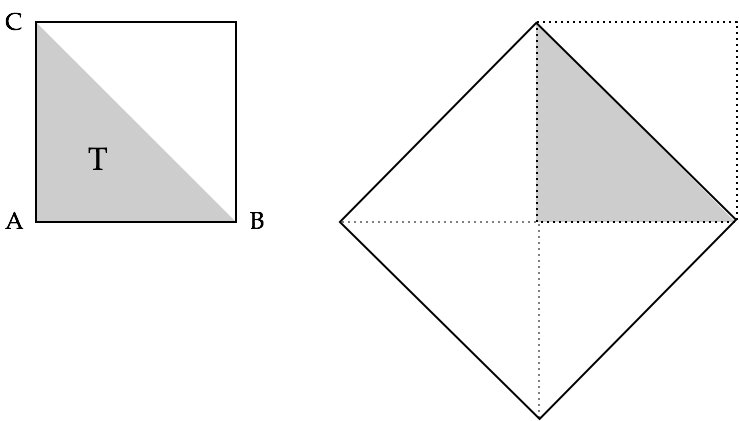
\includegraphics[scale=0.35]{FiguresArithmetic/UnitSquareSQRT2}
\caption{A pictorial schematic proof of The Pythagorian Theorem for
  the special case of an isosceles right triangle.
\label{fig:unitsquare}}
\end{center}
\end{figure}

\ignore{\Arny Please edit the figure to follow this story ... label the
  vertices of triangle $T$.  Any other labels? ... hypotenuse?  }

Say that the angle at vertex $A$ of $T$ is a {\em right angle},
\index{right angle} i.e., that its measure is $90^\circ$ ($90$ degrees
or, equivalently, $\pi/2$ radians).  In this case, we say that $T$ is
a {\em right triangle} \index{right triangle}.  Because $T$ is a right
triangle, the line from vertex $A$ to vertex $B$ and the line from
vertex $A$ to vertex $C$ are called the {\em sides} \index{side of a
  right triangle} (or the {\it legs}) of $T$, while the line from
vertex $B$ to vertex $C$ is called the {\em hypotenuse}
\index{hypotenuse of a right triangle} of $T$.  Triangle $T$ is {\em
  isosceles} \index{isosceles triangle} precisely when its two sides
have the same length.  The grey triangle in Fig.~\ref{fig:unitsquare}
is an isosceles right triangle.

\begin{theorem}[{\bf The Pythagorean Theorem}]
\label{thm:Pythagorean-thm}
Let $T$ be a right triangle whose two sides have respective lengths
$s_1$ and $s_2$, and whose hypotenuse has length $h$.  Then
\[ h^2 \ = \ s_1^2 + s_2^2. \]
Consequently, when $T$ is an {\em isosceles} right triangle, then $h^2
= 2 s_1^2$.
\end{theorem}

\ignore{\Denis I put here a figure for proving the result, may be it
  is not at the right place, feel free to put it elsewhere... I
  developed later a graphical proof of the theorem...}

The special case of the Pythagorean Theorem, which deals with
isosceles right triangles admits the very perspicuous proof presented
pictorially in Fig.~\ref{fig:unitsquare}.  Let us review this proof.

We begin with the unit-side square $S$ on the left of the figure.  We
partition $S$ by its diagonal into two unit-side isosceles right
triangles, one grey and one white.  Note that in this construction the
diagonal of $S$ is the (common) hypotenuse of the two triangles.  On
the righthand side of Fig.~\ref{fig:unitsquare}, we use our
partitioned version of $S$ to construct a new, bigger square, call it
$\widehat{S}$, whose side-length is the hypotenuse-length of the grey
triangle.  The dotted lines in the figure tell us how big
$\widehat{S}$ is (measured in area).
\begin{itemize}
\item
Square $S$ is unit-sided, hence has unit area.
\item
The grey triangle is half of $S$, hence has area $1/2$.
\item
Square $\widehat{S}$ is built from four copies of the grey
triangle, hence has area $4 \times 1/2 \ = \ 2$.
\end{itemize}
Because the hypotenuse of the grey triangle is a side of an area-$2$
square, we have just proved the following special case of the
Pythagorean Theorem.

{\em The hypotenuse of the unit-side isosceles right triangle has
  length $\sqrt{2}$.}
\[ \approx \approx \approx \approx \approx \approx \approx \approx \approx \approx \]

As part of the same movement toward formal mathematics, the
Sicilian-based Greek mathematician and polymath Archimedes
\index{Archimedes}
%
was systematically observing that squares are better approximations to
circles than triangles are; regular pentagons are better than squares;
regular hexagons are better than pentagons; and so on.  
Fig.~\ref{fig:approxcircle} illustrates this evidence
\ignore{\Denis I added a figure here, feel free to remove it if you
  believe it is not appropriate. I can also extend the figure with
  higher degree polygons....} 
\begin{figure}[htb]
\begin{center}
       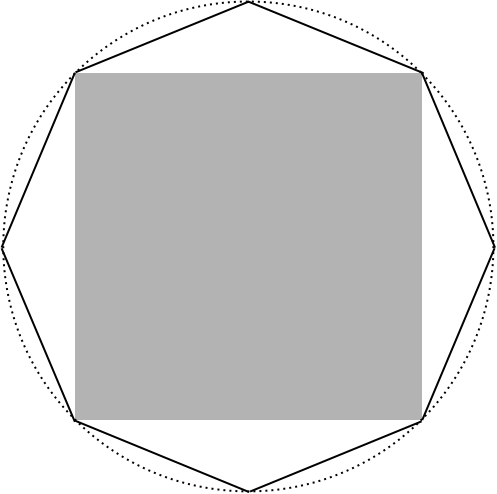
\includegraphics[scale=0.25]{FiguresArithmetic/ApproxCircle}
\caption{{\it Octagons approximate circles much better than squares do.}
\label{fig:approxcircle}}
\end{center}
\end{figure}
In fact, observed Archimedes, as the number of sides, $n$ in a regular
polygon grows without bound (or, as we might say today, tends to
infinity), each increase in $n$ brings a regular polygon closer to
being a circle.

In order to pursue their respective observations to their completion,
both Euclid and Archimedes would have to leave the world of the
rationals and enter the world of the {\it real numbers}
\index{number!real}
(so named by the French mathematician-philosopher Ren\'{e} Descartes).
\index{Descartes, Ren\'{e}}
It would take roughly two-thousand years from the time of Euclid and
Archimedes before the real numbers were {\em formally} introduced to
the world, by mathematical luminaries such as the early 19th-century
French mathematician-scientist Augustin-Louis Cauchy
\index{Cauchy, Augustin-Louis}
and the late 19th-century German mathematician Richard Dedekind.
\index{Dedekind, Richard}
It turned out to be much easier to recognize instances of non-rational
real numbers than to formally delimit the entire family of such
numbers.  Once again, happily, one could develop the real numbers in a
way that allowed one to view a rational number as a special type of
real number.  

During the millennia between the discoveries of Euclid, Archimedes, and
their friends and the full development of the real numbers,
mathematics was enriched repeatedly by the discovery of new conceptual
structures.  One of these---polynomials
\index{polynomial}
and their
\index{polynomial!root}
%
roots---ultimately led to the final major subsystem of our number
system.  In Chapter~\ref{sec:function}, we discussed the important
notion of {\em function}.  Polynomials \index{polynomial} are a
practically important class of functions that are delimited by the
operations needed to compute them.  Specifically, an $n$-argument
polynomial function---typically just called a polynomial---is a
function $P(x_1, x_2, \ldots, x_n)$ whose values can be calculated
using just the basic operations of arithmetic: addition/subtraction
and multiplication/division.\footnote{We pair the operations in this
  way because addition and subtraction are {\em mutually inverse
  operations},
\index{mutually inverse operations}
 as are multiplication and division.  This means that one can undo an
 operation (say, an addition) by performing its inverse operation (in
 this case, a subtraction).}
An argument that causes a polynomial function to {\it vanish}---i.e.,
assume the value $0$ is called a {\it root} of the polynomial.
\index{polynomial!root}
Here are a few simple, yet illustrative, examples:

\smallskip

\begin{tabular}{|c|c|c|}
\hline
 & Polynomial & Root(s) \\
\hline
1 &
$x+1$  &  $x= -1$ \\
2 &
$x-1$  &  $x= 1$ \\
3 &
$x^2 + 2x +1 = (x+1)^2$ & $x = -1$ \\ 
4 &
$x^2 - 2x +1 = (x-1)^2$ & $x = 1$ \\ 
5 &
$x^2 - 1$ & $x = 1$ and $x= -1$ \\
6 &
$x^2 + 1$ & {\em NO REAL ROOT} \\
7 &
$x^2 -2$  & $x = \sqrt{2}$ and $x = - \sqrt{2}$ \\
8 &
$x^2 + 2$ & {\em NO REAL ROOT} \\
\hline
\end{tabular}

\smallskip

\noindent
There are lessons, both major and minor, to be gleaned from this
table.

\noindent
($a$) Entries 3 and 4 illustrate that even simple polynomials can often be
written in several different ways.  These entries illustrate also that
roots can occur {\em with multiplicity:}
\index{polynomial!root!multiplicity}
one can view the value $x = -1$ as causing the polynomial $x^2 + 2x +1
= (x+1)\cdot (x+1)$ to vanish in two ways---once by setting the
lefthand factor $x+1$ to $0$ and once by setting the righthand factor
$x+1$ to $0$.

\noindent
($b$) Entries 5 and 7 illustrate that polynomials can have multiple
distinct roots.

\noindent
($c$) Perhaps most importantly, entries 6 and 8 illustrate that
polynomials can fail to have any real roots---even polynomials whose
expressions involve only positive integers!
\medskip

{\ignore {\Denis It is interesting here to stress how hard it was to solve such equations. Algebra raised only in the second half of the last millenium.
However, there are several nice examples of geometrical solutions.
One of the oldest comes from babylonians in the 18th century BC.
The numeral system was in base 60, and the problem was to determine the length of the side of a square which was part of a larger rectangle.
The following figure details the process.}}
{\Denis Add here a small introduction about solving polynomial of degree 2 from El Kwharizmi, or remove it and put it as an exercice.}
\begin{figure}[htb]
\begin{center}
       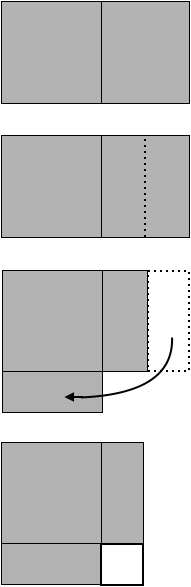
\includegraphics[scale=0.4]{FiguresArithmetic/tabletteMesopotamie}
\caption{{\it Solving $x^2 + x = 45$.
The idea of the proof is to represent the left hand side by the square $x^2$ beside a rectangle $60 \times x$.
Then, split the right rectangle into two equal parts and move one part a the bottom of the left square.
The final figure shows the whole square whose surface is equal to $45$ plus the surface of the white square
whose surface is equal to $30 \times 30$.
In base $60$, this is $15$. 
$45+15 = 60$, thus, the big square is the unit square, its side is $60$.
Thus, the length of the initial square is equal to $60-30=30$.}
\label{fig:equationBabillon}}
\end{center}
\end{figure}

\[ \approx \approx \approx \approx \approx \approx \approx \approx \approx \approx \]
{\em
We know that the problem here is actual because the square of a real
number can never be negative.
}
\[ \approx \approx \approx \approx \approx \approx \approx \approx \approx \approx \]
The absence of real roots for polynomial was considered a serious
deficiency on our number system.  The reaction to this deficiency was
similar in kind to all earlier recognized deficiencies.  A way was
found to expand the number system.  In this case, the expansion  was
based in the invention of a new {\it imaginary} number,
\index{number!imaginary}
so designated by Descartes.  This new number was named $i$
\index{imaginary number $i = \sqrt{-1}$}
(for ``imaginary'') and was defined to be a root of the polynomial
$P_{-1}(x) = x^2 +1$.  The number $i$ was evocatively often defined
via the equation, $i = \sqrt{-1}$.  By keeping our extended arithmetic
consistent with our former arithmetic, $-i$ also became a root of
$P_{-1}(x)$.  By combining the imaginary number $i$ with the real
number system, the {\it complex numbers}\index{number!complex} were
born.

Thankfully, the imaginary number $i$ was all that was needed to mend
the observed deficiency in the real numbers.  The complex numbers were
shown to be {\it algebraically complete}
\index{number!complex!algebraically complete}
in the sense expressed in the {\it Fundamental Theorem of Algebra}:
\index{Fundamental Theorem of Algebra}

\begin{theorem}[{\bf The Fundamental Theorem of Algebra}]
\label{thm:fund-thm-algebra}
Every polynomial of degree $n$ with complex coefficients has $n$ roots
over the complex numbers.
\end{theorem}

The proof of Theorem~\ref{thm:fund-thm-algebra} is beyond the scope of
our introductory text, but the result is a notable milestone in our
21st-century culture.

Our historical tour is now complete, so we can---finally---begin to
get acquainted with our number system and the operations that bring it
to life in applications..

\section{Integers}
\label{sec:integers}

The most basic class of numbers are the {\it integers},
\index{number!integer}
which are also referred to as the {\it whole numbers}
\index{number!integer!whole number}
or the {\em counting numbers}.
\index{number!integer!counting number}
%
As suggested in our ``biography'' of our number system
(Section~\ref{sec:number-taxonomy}), integers are certainly the
numbers that our prehistoric ancestors employed in the earliest days
of our species.  This section is devoted to exploring some of the
basic properties of the class of integers.  The details we provide in
Section~\ref{sec:primes} regarding the building blocks of the
integers, the {\it prime numbers}, \index{number!prime} will prepare
the reader for myriad applications of the integers, including
important security-related applications.  Our introduction to {\it
  pairing functions}, \index{pairing functions} in
Section~\ref{sec:pairing}, will open the door toward myriad
applications of the integers that build on the ordering properties of
the integers, coupled with tools for encoding highly structured data
as integers.  We begin to explore the basics of the integers.

\subsection{The Basics of the Integers: The Number Line}
\label{sec:integer-number-line}
\index{number!the number line}
\index{number!integer!the number line}

We survey a number of the most important properties of the following
three sets, which collectively comprise ``the integers.''
\begin{itemize}
\item
The set $\Z$
\index{$\Z$: the set of all integers}
comprises {\em all integers}---the positive and negative integers and
zero ($0$).
\item
The set $\N$
\index{$\N$: the set of nonnegative integers}
comprises the {\em nonnegative integers}---the positive integers and
zero ($0$).
\item
The set $\N^+$
\index{$\N^+$: the set of positive integers}
comprises the {\em positive integers}.
\end{itemize}
There is no universal default when one refers to ``the integers'' with
no qualifying adjective; therefore, we shall always be careful to
indicate which set we are discussing at any moment---often by
supplying the set-name: $\Z$ or $\N$ or $\N^+$.

\subsubsection{Natural orderings of the integers}
\label{sec:natural-orderings}

Several essential properties of the sets $\Z$, $\N$, and $\N^+$ are
consequences of the integers' behaviors under their natural order
relations:
\begin{itemize}
\item
the two {\em less-than} relations:
  \begin{itemize}
  \item
the {\em strict} relation ($<$).  We articulate ``$a < b$'' as ``$a$
is (strictly) less than $b$'' or ``$a$ is (strictly) smaller than
$b$.''
  \item
the {\em nonstrict} relation ($\leq$).  We articulate ``$a \leq b$''
as ``$a$ is less than or equal to $b$'' or ``$a$ is no larger than
$b$.''
  \end{itemize}
\index{$<$: the strict less-than relation} \index{$\leq$: the nonstrict less-than relation}

\item
their {\em converses,} the {\em greater-than} relations:
  \begin{itemize}
  \item
the {\em strict} relation ($>$).  We articulate ``$a > b$'' as ``$a$
is (strictly) larger than $b$.''
  \item
the {\em nonstrict} relation ($\geq$).  We articulate ``$a \geq b$''
as ``$a$ is greater than or equal to $b$'' or ``$a$ is no smaller than
$b$.''
  \end{itemize}
\index{$>$: the strict greater-than relation}
\index{$\geq$: the nonstrict greater-than relation}
\end{itemize}
One sometimes encounters {\em emphatic} versions of the strict
relations: $a << b$ and $a >> b$ indicate that $a$ is, respectively,
{\em much smaller than} or {\em much larger than} $b$.
\index{$<<$: the emphatic strict less-than relation}
\index{$>>$: the emphatic strict greater-than relation}

The reader will note throughout the text that order within a number
system is among one's biggest friends when reasoning about the numbers
within the system.  \index{number!ordering of numbers}

\subsubsection{The order-related laws of the integers}
\label{sec:order-laws}

\paragraph{\small\sf A. Total order and the Trichotomy Laws}

The sets $\Z$, $\N$, and $\N^+$ are {\em totally ordered},
\index{number!integer!total order}
\index{integer!total order}
also termed {\em linearly ordered}
\index{number!integer!linear ordering}
\index{integer!linear ordering}.

\smallskip

These facts are embodied in the {\em Trichotomy Laws for integers}.
\index{number!integer!Trichotomy Laws}
\index{integer!Trichotomy Laws}
\index{Trichotomy Laws}

\medskip

{\it The Trichotomy Laws for integers}.

\smallskip

(a)
%
{\it For each integer $a \in \Z$, precisely one of the following is true.}

\hspace*{.2in} $a$ equals $0$: $(a=0)$ \ \ \ \ \ \
 $a$ is {\em positive}: $(a>0)$ \ \ \ \ \ \
 $a$ is {\em negative}: $(a<0)$

\smallskip

(b)
%
{\it For each integer $a \in \N$, precisely one of the following is true.}

\hspace*{.2in} $a$ equals $0$: $(a=0)$ \ \ \ \ \ \
 $a$ is {\em positive}: $(a>0)$

\smallskip

(c)
%
{\it For each integer $a \in \N^+$:}

\hspace*{.2in} $a$ is {\em positive}: $(a>0)$

\bigskip

Consequently:

\smallskip

(a')
$\Z$ can be visualized via the ($2$-way infinite) number line:
\index{number!the number line}
\[ \ldots, -3, \  -2, \ -1, \ 0, \ 1,\  2, \ldots \]

\smallskip

(b')
$\N$ can be visualized via the ($1$-way infinite) number line:
\[  0, \ 1, \ 2, \ 3, \ldots \]

\smallskip

(c')
$\N^+$ can be visualized via the ($1$-way infinite) number line:
\[  1, \ 2, \ 3, \ldots \]


\bigskip

The Trichotomy Laws can be expressed using arbitrary pairs of integers,
rather than insisting that one of the integers be zero.  For the set
$\Z$, for instance, this version of the Laws takes the following form:

{\it For any integers $a, b \in \Z$, precisely one of the following is
  true.}

\hspace*{.2in} $a$ equals $b$: $(a=b)$ \ \ \ \ \ \
 $a$ is less than $b$: $(a<b)$ \ \ \ \ \ \
 $a$ is greater than $b$: $(a>b)$


\paragraph{\small\sf B. Well-ordering}

The sets $\N$ and $\N^+$ are {\it well-ordered}.
\index{number!nonnegative integers!well-ordering}
\index{nonnegative integers!well-ordering}
\index{number!positive integers!well-ordering}
\index{positive integers!well-ordering}

\medskip

\noindent
{\it The Well-ordering law for nonnegative and positive integers}. \\
%
{\it Every subset of $\N$ or of $\N^+$ has a smallest element (under
  the ordering $<$).}



\paragraph{\small\sf C. Discreteness}

The set $\Z$ is {\it discrete}.
\index{number!integer!discreteness}
\index{integer!discreteness}

\medskip

\noindent
{\it The discreteness of the integers.} \\
%
{\it For every integer $a \in \Z$, there is no integer between $a$ and
  $a+1$; i.e., there is no $b \in \Z$ such that $a < b < a+1$.}


\paragraph{\small\sf D. The laws of ``between-ness''}

The set $\Z$ obeys the {\it ``Between'' Laws}
\index{number!integer!''Between'' laws}\index{integer!''Between'' laws}

\medskip

\noindent
{\it The ``Between'' laws for integers}. \\
%
{\it For any integers $a, b \in \Z$, there are finitely many $c \in
  \Z$ such that $a < c < b$.}

\smallskip

Any such $c \in \Z$ lies {\em between} $a$ and $b$ along the number
line, whence the name of the law.


\subsection{Divisibility and Indivisibility}
\label{sec:divisibility}

Let $m$ and $n$ be nonnegative integers---symbolically, $m, n \in \N$.
We use any of the following locutions to assert the existence of a
positive integer $q$ such that $n = m \cdot q$. 
\index{number!integer!divisor} \index{number!integer!divisibility}
\index{$m \mid n$: $m$ divides $n$}
\begin{itemize}
\item
$m$ {\it divides} $n$
\item
$m$ {\it is a divisor of} $n$
\item
$n$ {\it is divisible by} $m$
\item
$m \mid n$.
\end{itemize}
This section is devoted to studying the possible {\it divisibility}
relations between the integers $m$ and $n$.  We begin by noting some
general facts.
\begin{itemize}
\item
Every integer $m$ divides $0$.

This is because of the universal equations $m \cdot 0 = 0 \cdot m =
0$.  These same equations verify that $0$ {\em does not} divide any
integer.
\item
$1$ divides every integer.

This is because of the universal equation $1 \cdot m = m$.
\item
Every nonzero integer divides itself.

This is because of the universal equation $m \cdot 1 = m$.
\end{itemize}

Some nonzero integers have many distinct divisors, while some have
very few.  Consider, for illustration, the first twelve positive
integers.
\[ \begin{array}{|c|c|}
\hline
\mbox{Number} & \mbox{Divisors} \\
\hline
\hline
1  &  \{ 1 \} \\
2  &  \{ 1, 2 \} \\
3  &  \{ 1, 3 \} \\
4  &  \{ 1, 2, 4 \} \\
5  &  \{ 1, 5 \} \\
6  &  \{ 1, 2, 3 \} \\
7  &  \{ 1, 7 \} \\
8  &  \{ 1, 2, 4, 8 \} \\
9  &  \{ 1, 3, 9 \} \\
10  & \{ 1, 2, 5, 10 \} \\
11  & \{ 1, 11 \} \\
12  & \{ 1, 2, 3, 4, 6, 12 \} \\
\hline
\end{array}
\]
But, note that all nonzero integers have at least $1$ and themselves
as divisors.  These ``sparsely divisible'' integers, which have only
two divisors, are called {\it primes}\index{numbers!integers!prime}
or {\it prime integers} or {\it prime numbers}; we study these
``building blocks of the positive integers'' in some detail in
Section~\ref{sec:primes}.

Before we turn to the primes we note that there is much of interest to
discuss about \index{numbers!integers!composite} nonprime---or, {\it
  composite}---integers, particularly, when we study pairs of
integers.  The next section looks at the defining property of
composite integers, namely, {\em divisibility}.

%times a two integers are perfectly divisible, sometimes divisibility
%goes wrong.  Let us investigate this in the next two sections.

\subsubsection{Divisibility and divisors}
\label{sec:divisibility+GCD}

We begin to study the several important aspects of integer
divisibility by considering a variety of simple, yet significant,
consequences of an integer $n$'s being divisible by an integer $m$.
We leave the following applications of the basic definitions as
exercises for the reader.

\begin{prop}
\begin{enumerate}
\item
If $m$ divides $n$, then $m$ divides all integer multiples of $n$.
Symbolically: If $m \mid n$, then $m \mid cn$ for all integers $c$.
\item
The relation ``divides'' is {\em transitive}; see
Chapter~\ref{sec:order-relation}.  Specifically, if $m$ divides $n$,
and $n$ divides $q$ for some integer $q$, then $n$ divides $q$.
\item
The relation ``divides'' distributes over addition.\footnote{We use
  the term ``distributes'' in the sense of the Distributive Law; see
  Chapter~\ref{sec:Arithmetic-Laws}.C.}  Specifically, if $m$ divides
$n$, and $m \mid (n+q)$ for some integer $q$, then $m \mid q$.

Hint: $\displaystyle \frac{n+q}{m} \ = \ \frac{n}{m} + \frac{q}{m}$.

\item 
For any integer $c \neq 0$,
\[ \left[[m \mid n] \ \ \mbox{ if, and only if, } \ \  [cm \mid cn] \right]. \]
\end{enumerate}
\end{prop}

The following result follows from the preceding facts.

\begin{prop}
\label{thm:m-common-divisor-nq}
Given integers $m$, $n$, and $q$, if $m \mid n$ and $m \mid q$, then
$m \mid (sn + tq)$ for all integers $s$ and $t$.
\end{prop}

\begin{proof}
The statement's two divisibility relations mean that there exist
integers $k_1$ and $k_2$ such that $k_1 \cdot m = n$ and $k_2 \cdot m
= q$.  By the distributive law, therefore:
\[ (k_1 \cdot s + k_2 \cdot t)m \ = \ sn+tq \]
for any $s$ and $t$.  \qed
\end{proof}

Proposition~\ref{thm:m-common-divisor-nq} points out a consequence of
integers $n$ and $q$ having a {\em common divisor} $m$.  \index{common
  divisor} A particularly consequential case occurs when $m$ is the
{\em greatest common divisor} of $n$ and $q$, \index{greatest common
  divisor} i.e., $m$ is the largest integer that divides both $n$ and
$q$.  We often refer to $m$ as the {\sc gcd} \index{{\sc gcd}: greatest
  common divisor} of $n$ and $q$ and use the notation
\[ m \ = \ \mbox{\sc gcd}(n, q) \]
to signal $m$'s having this status.

We are finally ready for our first major result about integer division
and divisors.


\begin{prop}[B\'{e}zout's identity]
\label{thm:gcd-n-linear}
For positive integers $n$ and $q$, {\sc gcd}$(n, q)$ is the smallest
positive linear combination of $n$ and $q$.
\index{B\'{e}zout, Etienne}

\noindent
Stated alternatively: For any positive integers $n$ and $q$, there
exist integers $s$ and $t$, not necessarily positive, such that
\[ sn + bq \ = \ \mbox{\sc gcd}(n, q). \]
\end{prop}

\begin{proof}
Consider the set of all integer linear combinations of $n$ and $q$:
\[  L_{n,q} \ \eqdef \   \{ sn +tq \ | \ s, s \in \Z \} \ \subseteq \ \Z. \]
Note that both $n$ and $q$ belong to $L_{n,q}$, because of the
respective cases $(s=1, t=0)$ and $(s=0, t=1)$.  One consequence of
this is that $L_{n,q}$ has a nonempty subset, call it
$L^{(>0)}_{n,q}$, all of whose elements are {\em positive} integers.

By the {\it Well-Ordering Principle of the positive integers}, the set
$L^{(>0)}_{n,q}$ has a smallest element, call it $m_0$.  By definition
of $L^{(>0)}_{n,q}$, $m_0$ is a positive integer, and there exist
integers $s_0$ and $t_0$ such that
\[  m_0 \ = \ s_0 n + t_0 q. \]

We claim that $L^{(>0)}_{n,q}$ in fact {\em consists precisely of all
  positive-integer multiples of $m_0$.}  Were this not the case, there
would be an element $rm$ of $L^{(>0)}_{n,q}$ that is not a
(positive-integer) multiple of $m_0$.  Let $m_1$ be the {\em smallest}
such element $m$.  We then have
\begin{enumerate}
\item
Because $m_1 \in L^{(>0)}_{n,q}$, there exist integers $s_1$ and $t_1$
such that
\[  m_1 \ = \ s_1 n + t_1 q. \]
\item
Because $m_0$ is the {\em smallest} element of $L^{(>0)}_{n,q}$, the
difference have $m_2 \ \eqdef \ m_1 - m_0$ must be positive, so that
$m_2 \ = \ (s_1 - s_0) n + (t_1 -t_0) q$ must belong to
$L^{(>0)}_{n,q}$.
\end{enumerate}
Now, we are in trouble because of the following incompatible facts.
\begin{itemize}
\item
On the one hand, $m_2$ {\em is not} a multiple of $m_0$!

If it were a multiple, then we would have $m_0$ dividing both $m_0$
(trivially) and $m_2 = m_1 - m_0$.  But this would imply that $m_0$
divides $m_1$, contrary to assumption.

\item
On the other hand,
$m_2$ {\em is} a multiple of $m_0$!

This is because $m_2 < m_1$, while $m_1$ is the {\em smallest} element
of $L^{(>0)}_{n,q}$ that is not a multiple of $m_0$.
\end{itemize}
This contradiction forces us to conclude that integer $m_1$ does not
exist; in other words: all elements of $L^{(>0)}_{n,q}$ are multiples
of $m_0$.

Let us summarize.  The set of positive integer linear combinations of
$n$ and $q$ consists entirely of integer multiples of a single integer
$m_0$.  This means, in particular, that $m_0$ is a common divisor
of $n$ and $q$.  The only way this situation could hold is if
$m_0 = \mbox{\sc gcd}(n,q)$, as claimed in the proposition.  \qed
\end{proof}

\ignore{******************

\textbf{Basic results and definitions}

{\Denis I used my notations, let see if you should change $a$ and $b$ to $n$ and $p$...}




\textbf{Greatest Common Divisor (GCD)}

\noindent {\bf Definition.} 
$GCD(a,b)$ is the largest number that is a divisor of both $a$ and $b$.
\bigskip




\bigskip

The proof considers $m$ as the smallest positive linear combination of
$a$ and $b$.  We prove respectively that $m \geq GCD(a,b)$ and $m \leq
GCD(a,b)$ by using the general previous properties.

\begin{enumerate}
\item 
By definition, $GCD(a,b) \mid a$ and $GCD(a,b) \mid b$, then, $GCD(a,b) \mid sa+tb$ for any $s$ and $t$ 
(and thus, in particular for the smallest combination). Then, $GCD(a,b)$ divides $m$ and $m \geq GCD(a,b)$.
\item
First, remark that $m \leq a$ because $a = 1.a + 0.b$ is a particular linear combination.
We show that $m \mid a$. 

By the division theorem, there exists a decomposition $a=q.m+r$ (where $0 \leq r<m$). 
Recall also that $m=sa+tb$ for some $s$ and $t$. 
Thus, $r$ can be written as $(1-qs)a+(-qt)b$ which is a combination of $a$ and $b$. 
However, as $m$ is the smallest, we get $r=0$.

Symmetrically $m$ divides also $b$.

Then, $m \leq GCD(a,b)$.
\end{enumerate}

***************}


\begin{corol}
Every linear combination of $n$ and $q$ is a multiple of $\mbox{\sc
  gcd}(n,q)$, and vice-versa.
\end{corol}


**HERE

**DEFINE EUCLIDEAN, SYNTHETIC DIVISION ... AND REMAINDERS.

\noindent {\bf Property}

 GCD(a,b) = GCD(b,rem(a,b))

In this last property, $rem$ denotes the reminder of the euclidian division of $a$ by $b$. 
It is detailed in the next section. 
The property is useful for quickly compute the $GCD$ of two numbers. 
This is in fact the basis of the well-known Euclid’s algorithm!

Proof.

The idea is to show that the set of common divisors of $a$ and $b$ (called $D$) is equal to the set
of the common divisors of $b$ and $rem(a,b)$ (called $D'$).
\begin{itemize}
\item If $d \in D$, $d \mid a$ and $d \mid b$.

As $a=q.b+rem(a,b)$, from property above above, we have $d \mid rem(a,b)$. Then, $d \in D'$.
\item If $d' \in D'$, $d' \mid b$ and $d' \mid rem(a,b)$.

From property $5$ above, $d'$ divides any linear combination of them, in particular $q.b+1.rem(a,b)$
thus,  $d' \mid a$ which proves that $d' \in D$.
\end{itemize}


There is a nice geometrical interpretation of the euclidian division and the CGD.
It corresponds to the largest surface unit to obtain a tessellation of the rectangle $a \times b$. 

%\begin{figure}[h]
%\begin{center}
%        \includegraphics[scale=0.5]{../FIGmaths/EuclideAlgo.pdf}
%        \caption{Geometric interpretation of the euclidian division of $a$ by $b$.
%        The first step is on the left, the second one on the right.}
%        \label{gcd}
%\end{center}
%\end{figure}


\subsubsection{Euclidian division}
\label{sec:euclidian}


Divisibility is not always perfect. 
As we learned in the elementary school, if one number does not evenly divide another, there is a remainder left over.
\medskip

\noindent {\bf Division theorem.}
Let $a$ and $b$ be two integers such that $b>0$, 
then there exists a unique pair of integers $q$ and $r$ such that $a=qb+r$ and $0 \leq r < b$.

Proving this theorem is two-fold: first the existence, and then the uniqueness.
{\Denis should we prove this or not? Would be fine, I put as follows - as a comment - a tentative proof, but I am not very happy with the phrasing}
%\begin{itemize}
%\item Let $E$ be the set of all positive integers in the form $n=a-b.z$.
%$E$ is not empty (well, for instance, it contains $a$) and $E \subset \mathds{N}$,
%thus, it has a smallest element. Let denote it $r$.
%
%We should now verify that $r<b$.
%It is easy by remarking that $r=a-b.z$ for some $z$ and $r-b$ does not belong to $E$
%because $r$ is the smallest one. Thus, $r-b <0$.
%\item Let us prove this part by contradiction. 
%Suppose there exist two such pairs of integers:
%$a=q_i.b + r_i$ for $i=1,2$.
%
%Then, $(q_1-q_2).b + r_1-r_2 = 0$.
%
%Thus, $b$ divides $r_1-r_2$ and $0 \leq r_1 < b$ and $0 \leq r_2 < b$
%
%$r_1-r_2 = 0$ and thus, $q_1=q_2$.
%\end{itemize}


\subsubsection{Prime numbers: building blocks of the integers}
\label{sec:primes}
\index{number!prime numbers}
\index{integers!prime numbers}

We single out a subclass of the positive integers whose mathematical
importance has been recognized for millennia but which have found
important applications (e.g., within the domain of computer security)
mainly within the past several decades.

**HERE
Thus, every positive
integer $n$ is divisible by $p=1$ (witnessed by $q=n$) and by $p=n$
(witnessed by $q=1$).

The class of integers we single out is defined by its divisibility
characteristics.

An integer $p >1$ is {\it prime}\index{number!integer!prime
  number}\index{number!integer!prime}\index{prime
  number}\index{integer!prime number}\index{integer!prime}
if its {\em only} positive integer divisors are $1$ (which divides
every integer) and itself (which is always a divisor).
\[ \approx \approx \approx \approx \approx \approx \approx \approx \approx \approx \]
{\em We often use the shorthand assertion, ``$p$ is a prime'' (or even
  the simpler ``$p$ is prime'') instead of the longer, but equivalent,
  ``$p$ is a prime integer.''}
\[ \approx \approx \approx \approx \approx \approx \approx \approx \approx \approx \]

  
\subsubsection{Primes as building blocks: The Fundamental Theorem of Arithmetic}
\label{sec:prime-factorization}

A very important way to classify a positive integer $n$ is to list the
primes that divide it, coupling each such prime $p$ with its {\it
multiplicity}, i.e., the number of times that $p$ divides $n$. 
Let $p_1, p_2, \ldots, p_r$ be all of the distinct primes that divide $n$,
and let each $p_i$ divide $n$ with multiplicity $m_i$.  The {\it prime
  factorization}
\index{prime factorization}
\index{integer!prime factorization}
\index{number!integer!prime factorization}
%
of $n$ is the product $p_1^{m_1} \cdot p_2^{m_2} \cdot \cdots \cdot
p_r^{m_r}$; note that this product satisfies the equation
\begin{equation}
\label{eq:prime-factorization}
n \ = \ p_1^{m_1} \cdot p_2^{m_2} \cdot \cdots \cdot p_r^{m_r}
\end{equation}

When writing an integer $n$'s prime factorization, it is traditional
to write the factorization in {\it canonical form},
\index{prime factorization!canonical form}
\index{integer!prime factorization!canonical form}
\index{number!integer!prime factorization!canonical form}
i.e., with the primes $p_1, p_2, \ldots, p_r$ that divide $n$ listed
in increasing order, i.e., so that $p_1 < p_2 < \cdots < p_r$.

\noindent
A positive integer $n$ is totally characterized by its canonical prime
factorization, as attested to by the following classical theorem,
which has been known for millennia and has been honored with the title
{\em The Fundamental Theorem of Arithmetic}.
\index{Fundamental Theorem of Arithmetic}
We state the Theorem in two equivalent ways which suggest different
ways of thinking about the result.

\begin{theorem}[The Fundamental Theorem of Arithmetic]
\index{Fundamental Theorem of Arithmetic}
\label{thm:Fund-Thm-Arith}

\noindent
{\rm (Traditional formulation.)}
%
The canonical prime factorization of every positive integer is unique.

\noindent
{\rm (Alternative formulation.)}
%
Let $n \in \N^+$ be a positive integer, and let $\widehat{P}_n$ denote the
ordered sequence of prime numbers that are no larger than $n$:

\begin{tabular}{ll}
$\widehat{P}_n \ =$  & $\langle P_1, \ P_3, \ \ldots, \ P_{r-1}, \ P_r \rangle$ \\
where:               & $P_1 \ = \ 2$ \\
                     & each  \ \ $P_i \ < \ P_{i+1}$ \\
                     & $P_r \ \leq \ n$.
\end{tabular}

\noindent
There exists a unique sequence of {\em nonnegative} integers, 
$\langle a_1, a_2, \ldots, a_r \rangle$
such that
\[
n \ = \ \prod_{i=1}^r \ P_i^{a_i} \ = \
P_1^{a_1} \cdot P_2^{a_2} \cdot \ \cdots \ \cdot P_{r-1}^{a_{r-1}} \cdot P_r^{a_r}
\]
\end{theorem}

A simple, yet important, corollary of Theorem~\ref{thm:Fund-Thm-Arith}
is the following result, whose proof we leave to the reader.

\begin{prop}
\label{thm:prime-divisor}
Every positive integer is divisible by at least one prime number.
\end{prop}


\subsubsection{Proving the Fundamental Theorem of Arithmetic}
\label{sec:FTA-proof}

The proof of Theorem~\ref{thm:Fund-Thm-Arith} is actually rather
elementary, providing that one approaches it gradually.  It employs a
lot of important techniques and concepts involved in ``doing
mathematics'', as discussed in the eponymous
Chapter~\ref{ch:doingmath}.

We begin with a purely technical result.

\begin{prop}
\label{thm:p-n-linear}
Let $p$ be a prime, and let $m$ be any positive integer that is {\em
  not} divisible by $p$.  There exist integers $a, b$, not necessarily
positive, such that
\[ ap + bm \ = \ 1. \]
\end{prop}

\begin{proof}
This result is a special case of Proposition~\ref{thm:gcd-n-linear}
because for any prime $p$ and integer $m$ that is not divisible by
$p$, {\sc gcd}$(p, m) = 1$.
\qed
\end{proof}

\begin{prop}
\label{thm:p-divides-onefactor}
If the prime $p$ divides a composite number $m \cdot n$, then either
$p$ divides $m$, or $p$ divides $n$, or both.\footnote{The closing
  phease ``or both'' signals our use of the {\em inclusive} or.}
\end{prop}

\begin{proof}
Let $p$, $m$, and $n$ be as asserted, and say that $p$ does not divide
$m$.  By Proposition~\ref{thm:p-n-linear}, then, there exist integers
$a, b$, not necessarily positive, such that
\[ ap + bm \ = \ 1. \]
Let us multiply both sides of this equation by $n$.  After some
manipulation---specfically, applying the distributive law---we find
that
\[ apn + bmn \ = \ n. \]
Now, $p$ divides the expression to the left of the equal sign: $p$
divides $p$ by definition, and $p$ divides $mn$ by assumption.  It
follows that $p$ must divide the expression to the right of the equal
sign---namely, the integer $n$.  \qed
\end{proof}

We are finally ready to develop the proof of the Fundamental Theorem.

\begin{proof}
{\small\sf The Fundamental Theorem of Arithmetic.}
%
Our dominant tool for proving Theorem~\ref{thm:Fund-Thm-Arith} will be
{\em proof by contradiction} (see Chapter~\ref{sec:Contradiction}).
We assume, for the sake of contradiction, that there is a positive
integer $n$ that has two distinct canonical prime factorizations.

Our argument will be a trifle simpler if we employ the {\em alternative} 
form of the Theorem.  To this end, let
\[ P_1 \ < \ P_2 \ < \cdots < \ P_{r-1} \ < \ P_r \]
denote, in increasing order, the set of all primes that do not exceed
$n$; i.e., every $P_i \leq n$.

The fact that $n$ has two distinct canonical prime factorizations
manifests itself, in this formulation, by the assumption that there
exist {\em two} distinct sequences of {\em nonnegative} integers, 
\[ \langle a_1, a_2, \ldots, a_r \rangle \ \ \ \mbox{ and } \ \ \
\langle b_1, b_2, \ldots, b_r \rangle 
\]
such that $n$ is expressible by---i.e., is equal to---both of the
following products of the primes $P_1$, $P_2$, \ldots, $P_{r-1}$, $P_r$.
\begin{eqnarray}
 & & 
\label{eq:product1.1}
P_1^{a_1} \cdot P_2^{a_2} \cdot \ \cdots \ \cdot P_{r-1}^{a_{r-1}}
\cdot P_r^{a_r} \\
 & &
\label{eq:product2.1}
P_1^{b_1} \cdot P_2^{b_2} \cdot \ \cdots \ \cdot P_{r-1}^{b_{r-1}}
\cdot P_r^{b_r}
\end{eqnarray}

Let us now ``cancel'' from the products (\ref{eq:product1.1}) and
(\ref{eq:product2.1}) the longest common prefix.  Because the two
products are, by hypothesis, distinct, at least one of them will not
be reduced to $1$ by this cancellation.  We are, therefore, left with
residual products of the forms
\begin{eqnarray}
 & &
\label{eq:product1.2}
P_i^{a_i} \cdot X \\
 & &
\label{eq:product2.2}
P_i^{b_i} \cdot Y
\end{eqnarray}
where:
\begin{itemize}
\item
Precisely one of $a_i$ and $b_i$ equals $0$.

Say, with no loss of generality (because we have no intrinsic way to
distinguish the products), that $b_i =0$ while $a_i \neq 0$.

\item
Products $X$ and $Y$ are composed only of primes that are strictly
bigger than $P_i$.
\end{itemize}
Note that 
\[ P_i^{a_i} \cdot X \ = \ P_i^{b_i} \cdot Y \ = \ Y, \]
because these products result from cancelling the same prefix from the
equal products (\ref{eq:product1.1}) and (\ref{eq:product2.1}), and
because $b_i =0$ so that $P_i^{b_i} = 1$.

We have finally reached the point of contradiction.

On the one hand, $P_i$ {\em must} divide the product $Y$, because it
divides the product $P_i^{a_i} \cdot X$ which equals $Y$.

On the other hand, $P_i$ {\em cannot} divide the product $Y$, because
every prime factor of $Y$ is bigger than $P_i$ (and a prime cannot
divide a bigger prime).

We conclude that one of the products (\ref{eq:product1.1}) and
(\ref{eq:product2.1}) cannot exist, so the theorem must hold.  \qed
\end{proof}



\subsubsection{A technical application: There are infinitely many primes}
\label{sec:infinite-primes}

The following result, which is traditionally attributed to the Greek
mathematician Euclid, \index{Euclid} one of the patriarchs of
mathematics, invokes Theorem~\ref{thm:Fund-Thm-Arith} in a crucial
way.

\begin{prop}
\label{thm:infinite-primes}
There are infinitely many prime numbers.
\end{prop}

\begin{proof}
Let us assume, for the sake of contradiction, that there are only
finitely many primes.  Say, in particular, that the following
$r$-element sequence enumerates all (and only) primes, in order of
magnitude:

\noindent
$\mbox{\bf Prime-Numbers} \ = \ 
\langle P_1, \ P_2, \ \ldots, \ P_r \rangle$

\noindent where
\[ P_1 \ < \ P_2 \ < \cdots < \ P_{r-1} \ < \ P_r \]
Of course, we know that the first several primes are
\[ (P_1 =2), \ (P_2 = 3), \ (P_3 =5), \ (P_4 = 7), \ (P_5 =11), \ldots \] 

We verify the {\em falseness} of the alleged completeness of the sequence
{\bf Prime-Numbers} by analyzing the positive integer
\[ n \ = \ 1 + \prod_{i=1}^r \ P_i \ = \ 1 \ + \ 
\left(P_1 \cdot P_2 \cdot \cdots \cdot P_r \right).
\]

We make three crucial observations.

\begin{enumerate}
\item
We note first that {\em the number $n$ is not divisible by any prime
number  in the sequence {\bf Prime-Numbers}.}

To see this, note that for each $P_k$ in the sequence,
\[
n / P_k \ = \ \frac{1}{P_k} \ + \ \prod_{i \neq k} \ P_i .
\]
Because $P_k \geq 2$, we see that $n / P_k$ obeys the inequalities
\[
\prod_{i \neq k} \ P_i \ < \ n/P_k \ < \ 1 + \prod_{i \neq k} \ P_i.
\] 
The discreteness of the set $\Z$---see
Section~\ref{sec:integer-number-line}---implies that $n / P_k$ is not
an integer, because it lies strictly between two adjacent integers.

\item
We note next that, because of assertion 1, if the sequence {\bf
  Prime-Numbers} actually did contain {\em all} of the prime numbers,
then we would have to conclude that {\em the number $n$ is not
  divisible by any prime number.}

\item
Finally, we remark that the Fundamental Theorem of Arithmetic
(Theorem~\ref{thm:Fund-Thm-Arith}) implies that {\em every integer is
  divisible by (at least one) prime number}.
\end{enumerate}
The preceding chain of assertions leads to a mutual inconsistency.  On
the one hand, the integer $n$ has no prime-integer divisor.  On the
other hand, no integer can fail to have a prime-integer divisor!

Let us analyze how we arrived at this uncomfortable place.
\begin{itemize}
\item
At the front end of this string of assertions we have the assumption
that there are only finitely many prime numbers.  We have (as yet) no
substantiation for this assertion.
\item
At the back end of this string of assertions, we have the ({\em rock
  solid}) Fundamental Theorem of Arithmetic
(Theorem~\ref{thm:Fund-Thm-Arith}).
\item
In between these two assertions we have a sequence of assertions, each
of which follows from its predecessors via irrefutable rules of
inference.
\end{itemize}
It follows that the {\em only} brick in this edifice that could be
faulty---i.e., the only assertion that could be false---is the initial
assumption, which states that there are only finitely many prime
numbers.  We must, therefore, conclude that this vulnerable assumption
is false!  In other words, we conclude from this classical proof by
contradiction that there are infinitely many prime numbers.  \qed
\end{proof}


\subsubsection{Applying the Theorem in {\em encryption}}
\label{sec:Primes-and-encryption}

One of the most important applications of Theorem~\ref{thm:Fund-Thm-Arith} is
as a mechanism for facilitating {\em encryption}.
\index{number!using the Fundamental Theorem of Arithmetic for encoding}
\index{number!using prime numbers for encoding}
\index{encoding sequences via the Fundamental Theorem of Arithmetic}
%
While the details of both encryption and the use of prime numbers to
that end are beyond the scope of this text, we will provide a peek
into that area by means of the following result concerning {\it
  encodings}.
\[ \approx \approx \approx \approx \approx \approx \approx \approx \approx \approx \]
{\em 
There is a crucial difference between {\em encoding} and {\em
  encryption}, despite the words' often being confused in the
vernacular.

Encoding involves a search for representations of objects, to achieve
some benefit, such as efficient computation or compactness.  An
example might be the conversion of Roman numerals to positional
numerals to enhance the arithmetic operations.

Encryption usually has some notion of secrecy attached.  An example
might be some key-based cipher which is intended to limit access to
someinformation.  }
\[ \approx \approx \approx \approx \approx \approx \approx \approx \approx \approx \]


sequences of positive integers as single integers!  This works as
follows.  Consider the (infinite) ordered sequence of {\em all primes:}
\[ (P_1 = 2), (P_2 = 3), (P_3 = 5), \ldots  \]
Let
\begin{equation}
\label{eq:sequence-vec-s}
\bar{s} \ = \ \langle m_1, m_2, \ldots, m_k \rangle
\end{equation}
be an arbitrary sequence of positive integers.  Then
Theorem~\ref{thm:Fund-Thm-Arith} assures us that the (single) positive
integer
\[ 
\iota(\bar{s}) \ \eqdef \ P_1^{m_1} \cdot P_2^{m_2} \cdot \ \cdots \
\cdot P_k^{m_k}
\]
is a (uniquely decodable) integer-representation of sequence $\bar{s}$.

We return to this idea of encoding-via-integers in a later chapter.

\subsubsection{Enrichment: The ``density'' of the prime numbers}
\label{sec:Prime-Number-Theorem}

{\Arny There are two advanced topics that we may want to
  mention/discuss: (1) The prime-number theorem ($n/ \log n$ primes
  $\leq n$); (2) the polynomials that generate lots of primes.  We
  should discuss this}


\subsection{Pairing Functions: Bringing Linear Order to Tuple Spaces}
\label{sec:pairing}
\index{pairing functions}

Paraphrasing an oft-used quip by the late stand-up comic Rodney
Dangerfield, integers ``don't get no respect''!  Superficially, it
appears that integers are useful for counting things but for little
else.  The Fundamental Theorem of Arithmetic
(Theorem~\ref{thm:Fund-Thm-Arith}) hints at the potential importance
of the prime numbers, but it does little to inspire respect for the
non-prime integers.  Once one augments the integers with a bit of
structure, {\em then} one can begin to represent interesting
situations.

As we shall see imminently, we can accomplish our goals by focusing on
very simple integer-based structures, namely, {\em ordered pairs of
  integers}---i.e.,
\index{integer!ordered pairs}
the sets $\Z \times \Z$, $\N \times \N$, and $\N^+ \times \N^+$.
Using $\Z \times \Z$ as the exemplar of these three sets of ordered
pairs of integers:
\begin{itemize}
\item
Each {\em element} of $\Z \times \Z$ has the form $\langle a_1, a_2
\rangle$, where $a_1$ and $a_2$ belong to $\Z$.
\item
The {\em semantics} of this set allow one to
  \begin{itemize}
  \item
{\em aggregate} any two elements of $\Z$, call them $b_1$, $\b_2$, and
create the ordered pair $\langle b_1, b_2 \rangle \in \Z \times \Z$;
  \item
given any pair $\langle a_1, a_2 \rangle \in \Z \times \Z$, {\em
  select} $a_1 \ \eqdef \ \mbox{first}(\langle a_1, a_2 \rangle)$ and
$a_2 \ \eqdef \ \mbox{second}(\langle a_1, a_2 \rangle)$.
  \end{itemize}
\end{itemize}

\subsubsection{Encoding complex structures via ordered pairs}
\label{sec:encodings-via-ordered-pairs}

Among the myriad other structures that ``contain'' integers that one
can represent---or, {\it encode}---via some sort of iterated formation
of ordered pairs are the following.

\noindent
(i) {\em (Ordered) tuples of integers.}\index{tuples of integers}\index{integer!tuples}\index{tuples of integers!via ordered pairs}\index{integer!tuples!via ordered pairs}
%
We focus on the set of $k$-tuples of integers, for any integer $k >
1$.  One way to accomplish this is by recursion, with {\em ordered
  pair} (the just-described case $k=2$) as the base case.  For any $k
> 1$, we represent the $k$-tuple $\langle a_1, a_2, \ldots, a_k
\rangle$ as the ordered pair whose {\em first} is the ordered
$(k-1)$-tuple $\langle a_1, a_2, \ldots, a_{k-1} \rangle$ and whose
{\em second} is the integer $a_k$:
\[ \langle a_1, a_2, \ldots, a_k \rangle \ \ = \ \
\langle \langle a_1, a_2, \ldots, a_{k-1} \rangle, a_k \rangle \]

\noindent
(ii) {\em Strings of integers.}\index{integer!string}\index{string of integers}\index{integer!string!via ordered pairs}\index{string of integers!via ordered pairs}
%
One way to represent the string of integers $a_1 a_2 \cdots a_n$ using
ordered pairs is as follows.
\[ a_1 a_2 \cdots a_n \ \ = \ \
\langle a_1, \langle a_2, \langle a_3, \ldots, \langle a_{n-2},  a_{n-1}
\rangle, a_n \rangle \cdots \rangle \rangle \rangle
\]
The following small example should make the aggregation perfectly
clear (without any possibly confusing dots):
\[ a_1 a_2 a_3 a_4 \ \ = \ \
\langle a_1, \langle a_2, \langle a_3,  a_4 \rangle \rangle \rangle
\]

\noindent
(iii) {\em Binary trees.}\index{integer!binary tree!via ordered pairs}\index{binary tree of integers!via ordered pairs}
%
For illustration, the {\em complete binary tree}\index{complete binary tree}\index{binary tree!complete}\index{complete binary tree!via ordered pairs}\index{binary tree!complete!via ordered pairs}
with leaves $a_1$, $a_2$, $a_3$, $a_4$, $a_5$, $a_6$, $a_7$, $a_8$
would be represented via the following aggregation of ordered pairs,
\[
\langle
\langle \langle a_1,  a_2 \rangle, \langle a_3,  a_4 \rangle \rangle,
\langle \langle a_5,  a_6 \rangle, \langle a_7,  a_8 \rangle \rangle
\rangle
\]
while the {\em comb-structured binary tree}\index{comb-structured binary tree}\index{comb-structured binary tree!via ordered pairs}
with the same leaves would be represented via the following
aggregation of ordered pairs,
\[
\langle a_1, \langle a_2, \langle a_3, \langle a_4, \langle a_5,
\langle a_6, \langle a_7, a_8 \rangle \rangle \rangle \rangle
\rangle \rangle \rangle
\]
\[ \approx \approx \approx \approx \approx \approx \approx \approx \approx \approx \]
{\em It should be no surprise that a single character string, such as
  $\langle a_1, \langle a_2, \langle a_3, a_4 \rangle \rangle
  \rangle$, can be used to represent many distinct, but {\em
    isomorphic} (literally, ``same-shaped''), objects---for instance a
  length-$4$ string and a $4$-leaf comb-structured binary tree.
  Indeed, one of the biggest strengths of mathematics is its ability
  to expose often-unexpected structural similarities.  }
\[ \approx \approx \approx \approx \approx \approx \approx \approx \approx \approx \]

\medskip

The rather long preamble to this section has been our attempt to
enhance the reputation of the integers---all three sets, $\Z$, $\N$,
and $\N^+$---in the eyes of the reader.  With that process hopefully
begun, we turn now to a demonstration via multiple examples that what
we have accomplished has largely been an exercise in form rather than
essence.  Specifically, we show that one can easily and efficiently
``encode'' structures exemplified by the ones we have been describing
as positive integers!

\medskip

\noindent
What does it mean to {\em encode} \index{encode} one class of
  entities, $A$ as another class $B$?  Our definition is a rather
  strict mathematical one.  We insist that there exist a {\em
    bijection} $F_{A,B}$ that maps $A$ {\em one-to-one onto} $B$ (cf.,
  Chapter~\ref{sec:function}).  In other words, when presented with an
  element $a \in A$, the function $F_{A,B}$ ``produces'' a unique
  element $b \in B$, and conversely, when presented with an element $b
  \in B$, the function $F^{-1}_{A,B}$ ``produces'' a unique element $a
  \in A$.

\subsubsection{Pairing functions: Bijections between $\N^+ \times \N^+$ and $\N^+$}
\label{sec:building-pairing-functions}

The remainder of this section is devoted to developing {\em easily
  computed} bijections between the set $\N^+ \times \N^+$ and the set
$\N^+$ of positive integers.  We thereby exhibit easily computed
mechanisms for \underline{encoding} ordered pairs of integers---hence,
also, tuples, strings, and binary trees of integers---as single
integers.  Because of the special role of ordered pairs of integers in
our study of encodings of structured sets of integers---they form the
fundamental puzzle from whose solution all else will follow---a
special name has been associated with bijections between $\N^+ \times
\N^+$ and $\N^+$.  These special bijections are called {\it pairing
  functions}.  \index{pairing functions!encodings}

One of the most valuable by-products of encodings provided by pairing
functions is that such encodings provide {\em linear orderings} of the
\index{pairing functions!linear orderings}
set being encoded.  We noted in Section~\ref{sec:integers}.A that
``order within a number system is among one's biggest friends when
reasoning about the numbers within the system.''  The orderings
provided by these encodings are particularly
valuable when the structured sets being encoded as integers do not
have their own ``intrinsic'' or ``natural'' orderings.  Included in
this category are  structures such as tuples,
strings, and trees.
\[ \approx \approx \approx \approx \approx \approx \approx \approx \approx \approx \]
Of course some structured sets do have natural, native linear orders:
consider, as one such, strings under lexicographic ordering.  Even for
such sets, we often benefit from having alternative orderings as we
design and analyze algorithms on the sets.
\[ \approx \approx \approx \approx \approx \approx \approx \approx \approx \approx \]

We focus on $\N^+$ as the avatar of {\it integer}, rather than on $\Z$
or $\N$, primarily for definiteness and a bit of clerical
simplification.  We could easily rewrite this section with a focus on
bijections between $\Z \times \Z$ and $\Z$ or on bijections between
$\N \times \N$ and $\N$.

\bigskip


We now embark on a very short guided tour that will introduce the
reader to three interesting pairing functions.

\paragraph{\small\sf A.The Diagonal pairing function $\d$}
\index{The Diagonal pairing function $\d$}

Pairing functions first appeared in the literature early in the 19th
century.  Perhaps the simplest and ``prettiest'' such function (since
it is a {\em polynomial}) appears, pictorially, in an 1821 work by the
great French mathematician Augustin Cauchy \cite{Cauchy21}.
\index{Cauchy, Augustin}
%
This {\em diagonal} pairing function was formally specified a
half-century later by the German logician Georg Cantor,
\index{Cantor, Georg}
%
whose studies \cite{Cantor74,Cantor78} revolutionized how we think
about {\em infinite} sets.

\begin{equation}
\label{eq:diag}
\d(x, y) \ = \
{{x+y-1} \choose 2} + (1-y)
\end{equation}
($\d$ of course has a twin that exchanges $x$ and $y$).  $\d$'s
mapping of $\N^+ \times \N^+$ onto $\N^+$, as depicted in
Fig.~\ref{fig:diag}, exposes that we can view $\d$'s mapping of $\N^+
\times \N^+$ as a two-step conceptual process:
\begin{figure}[htb]
\begin{center}
      \includegraphics[scale=0.4]{FiguresArithmetic/PairingDiagonal}
%\begin{tabular}{r|r|r|r|r|r|r|r|r}
% 1 &  3 &  6 & 10 & \fbox{15} &  21 &  28 &  36 & $\cdots$ \\
% 2 &  5 &  9 & \fbox{14} & 20 &  27 &  35 &  44 & $\cdots$ \\
% 4 &  8 & \fbox{13} & 19 & 26 &  34 &  43 &  53 & $\cdots$ \\
% 7 & \fbox{12} & 18 & 25 & 33 &  42 &  52 &  63 & $\cdots$ \\
%\fbox{11} & 17 & 24 & 32 & 41 &  51 &  62 &  74 & $\cdots$ \\
%16 & 23 & 31 & 40 & 50 &  61 &  73 &  86 & $\cdots$ \\
%22 & 30 & 39 & 49 & 60 &  72 &  85 &  99 & $\cdots$ \\
%29 & 38 & 48 & 59 & 71 &  84 &  98 & 113 & $\cdots$ \\
%$\vdots$ & $\vdots$ & $\vdots$ & $\vdots$ & $\vdots$ & $\vdots$ &
%  $\vdots$ & $\vdots$ & $\ddots$
%\end{tabular}
\end{center}
\caption{{\it The diagonal pairing function $\d$.  The shell $x+y = 6$
    is highlighted.}
\label{fig:diag}}
\end{figure}
\begin{enumerate}
\item
partitioning $\N^+ \times \N^+$ into ``diagonal shells'' defined as
\[
\{ \langle x,y \rangle \ | \ x+y = 2 \}, \ \ 
\{ \langle x,y \rangle \ | \ x+y = 3 \}, \ \ 
\{ \langle x,y \rangle \ | \ x+y = 4 \}, \ \ \ldots
\]
This is accomplished by the following subexpression in (\ref{eq:diag}).
\[
{1 \over 2} (x+y) \cdot (x+y-1) \ = \ {{x+y-1} \choose 2}
\]

\item
``climbing up'' these shells in order.

This is accomplished by the additional subexpression ``$+1-y$'' in
(\ref{eq:diag}).
\end{enumerate}
\[ \approx \approx \approx \approx \approx \approx \approx \approx \approx \approx \]
{\em Keep in mind that we have just described a {\em conceptual}
  process.  $\d$ is a function, {\em not} an algorithm.  ``Running''
  this infinite process would take forever.}
\[ \approx \approx \approx \approx \approx \approx \approx \approx \approx \approx \]
Understanding $\d$'s structure leads to a broadly applicable strategy
for inductively constructing a broad range of pairing functions.  We
develop this strategy in Subsection B, along with an accompanying
rather simple inductive verification of bijectiveness.  One finds a
computationally more satisfying proof of $\d$'s bijectiveness in
\cite{Davis58}, along with an explicit recipe for computing $\d$'s
inverse.  The material in \cite{Davis58} builds specifically on $\d$'s
structure.

\medskip

\[ \approx \approx \approx \approx \approx \approx \approx \approx \approx \approx \]
{\small\sf Esoterica for enrichment:}
{\em The fact that $\d$ is a {\em polynomial} in $x$ and $y$ raises
  the natural (to a mathematician!)~question of whether there exist
  any other polynomial pairing functions.  This is a quite advanced
  topic that is beyond the scope of this text.  Indeed, even as a
  research problem, the question remains largely open.  But, a few
  nontrivial pieces of an answer are known.}
\begin{enumerate}
\item
There is no {\em quadratic} polynomial pairing function other than
$\d$ (and its twin) \cite{FueterP23,LewR78a}.
\item
No {\em cubic} or {\em quartic} polynomial is a pairing function
\cite{LewR78b}.
\item
The development in \cite{LewR78b} excludes large families of
higher-degree polynomials from being pairing functions; e.g., a {\em
  super-quadratic} polynomial whose coefficients are all positive
cannot be a pairing function.
\end{enumerate}
\[ \approx \approx \approx \approx \approx \approx \approx \approx \approx \approx \]

\paragraph{\small\sf B. Enrichment: A methodology for constructing pairing functions}
\index{constructing pairing functions via ``shells''}
\index{pairing functions as storage mappings for arrays/tables}

The shell-oriented strategy that underlies the diagonal pairing
function $\d$ can be adapted to incorporate shell-``shapes'' that are
inspired by a variety of computational situations---and can be applied
to great computational advantage in such situations.  We describe how
such adaptation can be effected, and we describe a few explicit shapes
and situations.  We invite the reader to craft others.

\medskip

\noindent {\underline{\bf Procedure}} {\small\sf PF-Constructor}($\a$) \\
/*Construct a shape-inspired pairing function (PF) $\a$*/
\begin{description}
\item[Step 1.]
%
Partition the set $\N^+ \times \N^+$ into finite sets called {\it
  shells}.  Order the shells linearly in some way: many natural
shell-partitions carry a natural order.
\end{description}
As noted above, Shell $c$ of the diagonal pairing function $\d$ is the
following subset of $\N^+ \times \N^+$: $\{ \langle x,y \rangle \ |
\ x+y = c \}$.  The parameter $c$ orders $\d$'s shells.

\begin{description}
\item[Step 2.]
Construct a pairing function from the shells as follows.
  \begin{description}
  \item[Step 2a.]
Enumerate $\N^+ \times \N^+$ shell by shell, honoring the ordering of
the shells; i.e., list the pairs in shell \#1, then shell \#2, then
shell \#3, etc.
  \item[Step 2b.]
Enumerate each shell in some systematic way, e.g., ``by columns'':
Enumerate the pairs $\langle x,y \rangle$ in each shell in increasing
order of $y$ and, for pairs having equal $y$ values, in decreasing
order of $x$.
  \end{description}
\end{description}

\begin{prop}
\label{thm:PF-construct}
Any function $\a: \N^+ \times \N^+ \leftrightarrow \N^+$ that is
designed via Procedure {\small\sf PF-Constructor} is a bijection.
\end{prop}

\begin{proof}(Sketch) Step 1 of Procedure {\small\sf PF-Constructor}
constructs a partial order on $\N^+ \times \N^+$, in which: ($a$) each
shell is finite; ($b$) there is a linear order on the shells.  Step 2
extends this partial order to a linear order, by honoring the inherent
ordering of shells and imposing a linear order within each shell.  The
function constructed via the Procedure is: {\em injective} because the
disjoint shells are enumerated sequentially; {\em surjective} because
the enumeration within each shell begins immediately after the
enumeration within the preceding shell, with no gap.  \qed
\end{proof}

\bigskip

We have noted how to use Procedure {\small\sf PF-Constructor} to
construct pairing function $\d$.  We now use the Procedure to design
two other useful pairing functions.

\paragraph{\small\sf C. The Square-shell pairing function $\s$}
\index{The Square-shell pairing function $\s$}

One computational situation where pairing functions can be useful
involves storage-mappings for arrays/tables that can expand and/or
contract dynamically.  In conventional systems, when one expands an $n
\times n$ table into an $(n+1) \times (n+1)$ table, one allocates a
new region of $(n+1)^2$ storage locations and copies the current table
from its $n^2$-location region to the new region.  Of course, this is
very wasteful: one is moving $\Omega(n^2)$ items to make room for the
anticipated $2n+1$ new items.  On any given day, the practical impact
of this waste depends on current technology.  But, this is a
mathematics text, not an engineering one, so we are exploring whether
{\em in principle} we can avoid the waste.  The answer is ``YES''.  If
we employ a pairing function $\varepsilon: \N^+ \times \N^+
\leftrightarrow \N^+$ to allocate storage for tables, then to expand a
table from dimensions $n \times n$ to $(n+1) \times (n+1)$, we need
move only $O(n)$ items to accommodate the {\em new} table entries; the
current entries need not be moved.  For square tables, the following
{\it Square-shell} pairing function $\s$ manages the described
scenario perfectly.  After describing $\s$, we comment on managing
tables of other shapes.
\begin{figure}[htb]
\begin{center}
%\begin{tabular}{r|r|r|r|r|r|r|r|r}
%  1 &  4 &  9 & 16 & \fbox{25} &  36 &  49 &  64 & $\cdots$ \\
%  2 &  3 &  8 & 15 & \fbox{24} &  35 &  48 &  63 & $\cdots$ \\
%  5 &  6 &  7 & 14 & \fbox{23} &  34 &  47 &  62 & $\cdots$ \\
% 10 & 11 & 12 & 13 & \fbox{22} &  33 &  46 &  61 & $\cdots$ \\
%\fbox{17} & \fbox{18} & \fbox{19} & \fbox{20} & \fbox{21} &  32 &  45
%  &  60 & $\cdots$ \\ 
% 26 & 27 & 28 & 29 & 30 &  31 &  44 &  59 & $\cdots$ \\
% 37 & 38 & 39 & 40 & 41 &  42 &  43 &  58 & $\cdots$ \\
% 50 & 51 & 52 & 53 & 54 &  55 &  56 &  57 & $\cdots$ \\
%$\vdots$ & $\vdots$ & $\vdots$ & $\vdots$ & $\vdots$ & $\vdots$ &
%  $\vdots$ & $\vdots$ & $\ddots$
%\end{tabular}
   \includegraphics[scale=0.4]{FiguresArithmetic/PairingSquareShell}
\end{center}
\caption{{\it The square-shell pairing function $\s$.  The shell
    $\max(x,y) = 5$ is highlighted.}
\label{fig:pairingSquareShell}}
\end{figure}
\begin{equation}
\label{e.square}
\begin{array}{ccl}
\s(x, y) & = & m^2 + m + y-x+1 \\
 & & \mbox{where } \ \ \  m \ \eqdef \ \max(x-1,y-1).
\end{array}
\end{equation}
One sees in Fig.~\ref{fig:pairingSquareShell} that $\s$ follows the
prescription of Procedure PF-Constructor: (1) it maps integers into
the ``square shells'' defined by: $m = 0, \ m = 1, ...$.  (2) it
enumerates the entries in each shell in a counterclockwise direction.
(Of course, $\s$ has a twin that enumerates the shells in a clockwise
direction.)
\[ \approx \approx \approx \approx \approx \approx \approx \approx \approx \approx \]
{\em Using somewhat more complicated instantiations of Procedure
  PF-Constructor, the study in \cite{Rosenberg75} adapts the
  square-shell pairing function $\s$ to: ($a$) accommodate, with no
  wastage, arrays/tables of any fixed aspect ratio $an \times bn$
  ($a,b \in \N$); ($b$) accommodate, with only $O(n)$ wastage,
  arrays/tables whose aspect ratios come from a fixed finite set of
  candidates---i.e., $(a_1 n \times b_1 n)$ or $(a_2 n \times b_2 n)$
  or \ldots or $(a_k n \times b_k n)$.}
\[ \approx \approx \approx \approx \approx \approx \approx \approx \approx \approx \]

\paragraph{\small\sf D. The Hyperbolic-shell pairing function $\h$}
\index{The Hyperbolic-shell pairing function $\h$}

We have just seen, in subsections B and C, that when the growth
patterns of one's arrays/tables is very constrained, one can use
pairing functions as storage mappings with very little wastage.  In
contrast, if one employs a pairing function such as $\d$ without
consideration of its wastage, then a storage map would show some
$O(n)$-entry tables being ``spread'' over $\Omega(n^2)$ storage
locations.  In the worst-case, $\d$ spreads the $n$-position $1 \times
n$ array/table over $> {1 \over 2} n^2$ addresses: $\d(1,1) = 1$ and
$\d(1,n) = {1 \over 2} (n^2 + n)$.  This degree of wastefulness can be
avoided via careful analysis, coupled with the use of Procedure
PF-Constructor.  The target commodity to be minimized is the {\it
  spread} of a PF-based storage map, which we define as follows.
\index{the spread of a pairing function}

Note that an ordered pair of integers $\langle x,y \rangle$ appears as
a position-index within an $n$-position table if, and only if, $xy
\leq n$.  Therefore, we define the spread of a PF-based storage map
$\m$ via the function
\begin{equation}
\label{e.compact}
{\bf S}_{\cal M}(n) \ \eqdef \ \max\{ \m(x, y) \ | \ xy \leq n \}.
\end{equation}
${\bf S}_{\cal M}(n)$ is the largest ``address'' that PF $\m$ assigns
to any position of a table that has $n$ or fewer positions.

Happily, the tools we have developed enable us to design a pairing
function that (to within constant factors) has minimum worst-case
spread.  This is the {\em Hyperbolic-shell pairing function} $\h$ of
(\ref{e.hyper}) and Fig.~\ref{fig:pairingHyper}.\footnote{Details appear in
  \cite{Rosenberg74,Rosenberg75}.}
\begin{equation}
\label{e.hyper}
\begin{array}{lcll}
\multicolumn{4}{l}{\mbox{Let $\delta(k)$ be the number of divisors of
    the integer $k$.}} \\
\h(x,y) & = & {\displaystyle \sum_{k=1}^{xy-1} \delta(k) \ \ +} &
  \mbox{the position of } \ \langle x, y \rangle \ \mbox{ among 2-part} \\
        &   &  & \mbox{factorizations of the number $xy$, in} \\
        &   &  & \mbox{reverse lexicographic order}
\end{array}
\end{equation}
\begin{figure}[htb]
\begin{center}
%\begin{tabular}{r|r|r|r|r|r|r|r}
% 1 &  3 &  5 &   8 &  10 & \fbox{14} &  16  & $\cdots$ \\
% 2 &  7 & \fbox{13} &  19 &  26 &  34 &  40 & $\cdots$ \\
% 4 & \fbox{12} & 22 &  33 &  44 &  56 &  69 & $\cdots$ \\
% 6 & 18 & 32 &  48 &  64 &  81 &  99  & $\cdots$ \\
% 9 & 25 & 43 &  63 &  86 & 108 & 130  & $\cdots$ \\
%\fbox{11} & 31 & 55 &  80 & 107 & 136 & 165 & $\cdots$ \\
%15 & 39 & 68 &  98 & 129 & 164 & 200  & $\cdots$ \\
%17 & 47 & 79 & 116 & 154 & 193 & 235  & $\cdots$ \\
%$\vdots$ & $\vdots$ & $\vdots$  & $\vdots$ & $\vdots$ &
%  $\vdots$ & $\vdots$ & $\ddots$
%\end{tabular}
      \includegraphics[scale=0.4]{FiguresArithmetic/PairingHyper}
\end{center}
\caption{{\it The hyperbolic pairing function $\h$.  The shell $xy = 6$ is
highlighted.}
\label{fig:pairingHyper}}
\end{figure}


\begin{prop}[\cite{Rosenberg75}]
\label{thm:hyp-opt}
{\bf (a)}
The hyperbolic function $\h$ is a pairing function.

\noindent {\bf (b)}
The spread of $\h$ is given by
${\bf S}_{\cal H}(n) \ = \ O(n \log n)$.\footnote{A  detailed
  analysis reveals that the spread of $\cal H$ is closely related to
  the {\em natural} logarithm, whose base is Euler's constant $e$.}

\noindent {\bf (c)}
No pairing function has better compactness than $\h$ (in the worst
case) by more than a constant factor.
\end{prop}

\begin{proof}
{\bf (a)} The fact that $\h$ is a pairing function follows from
Proposition~\ref{thm:PF-construct}.

\noindent {\bf (b)}
The pairing function $\h$ maps integers along the ``hyperbolic
shells'' defined by $xy = 1, \ xy =2, \ xy=3, \ldots$.  Hence,
when an integer $n$ is ``placed'' into the table of values of
$\h$, the number of occupied slots is within $n$ of
\[ \sum_{i=1}^{n-1} \ |\{ \langle x,y \rangle \ | \ xy < i \}| 
\]
Elementary calculations show that this sum is $O(n \log n)$.

\noindent {\bf (c)} The optimality of $\h$ in compactness (up to
constant factors) is seen via the following argument.  The set of
tables that have $n$ or fewer positions are those of aspect ratios
$a_i \times b_i$, where $a_i b_i \leq n$.  As one sees from
Fig.~\ref{f.hyp} (generalized to arbitrary $n$), the union of the
positions of all these arrays is the set of integer lattice points
under the hyperbola $xy = n$.  It is
well-known---cf.~\cite{NivenZ80}---that this set of points has
cardinality $\Theta(n \log n)$.\footnote{Recall from
  Chapter~\ref{sec:set-concepts} that the {\it cardinality} of a
  finite set $S$ is the number of elements in $S$.}  Since every table
contains position $\langle 1,1 \rangle$, it follows that, for every
$n$, some table containing $n$ or fewer positions is spread over
$\Omega(n \log n)$ ``addresses.''  \qed
\end{proof}
\begin{figure}[htb]
\begin{center}
       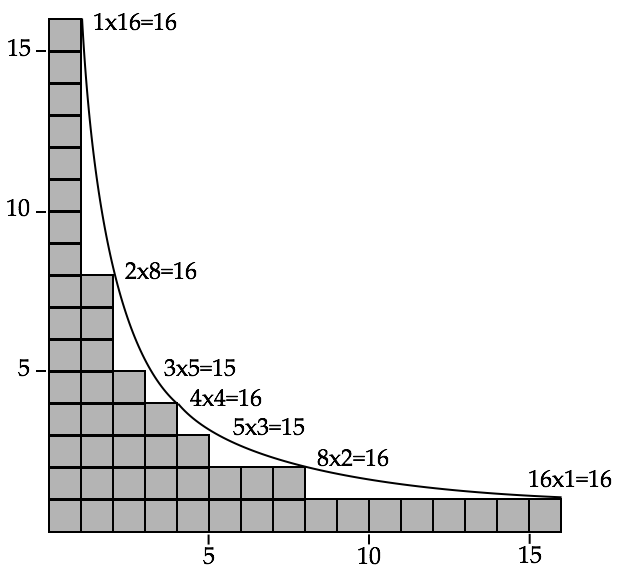
\includegraphics[scale=0.4]{FiguresArithmetic/PairingHyp}
\caption{The aggregate set of positions of tables having $16$ or
    fewer position.  To help the reader understand the figure, we
    include the curve $f(x,y) = xy$ which provides an upper envelope
    for the set.  A careful look at this curve will reveal that it
    touches the set of positions at the points $\langle x,y \rangle
    \in \{ \langle 1,16 \rangle, \ \langle 2,8 \rangle, \ \langle 4,4
    \rangle, \ \langle 8,2 \rangle, \ \langle 16,1 \rangle \}$, but it
    does {\em not} touch the set at the points $\langle x,y \rangle
    \in \{ \langle 3,5 \rangle, \ \langle 5,3 \rangle \}$. 
\label{f.hyp}}
\end{center}
\end{figure}

\subsubsection{There are {\em no more} ordered pairs than integers}
\label{sec:cardinality-NxN}

\paragraph{\small\sf A. Comparing infinite sets via cardinalities}
\index{cardinality!infinite set}

We have remarked earlier (and will do so again) that one must be very
careful when reasoning about infinite sets.  They can behave in ways
that seem quite contradictory to our experience with finite sets.  One
of the most dramatic instances of this is encountered when we ask
whether the set $\N^+ \times \N^+$ is ``larger'' than the set $\N^+$.
We need to put the word ``larger'' in quotes because we do not know
(yet) what the word means in the setting of infinite sets.  Supplying
a meaning for the word that is at once mathematically tractable and
intuitively plausible was among the seminal contributions of the
19th-century German mathematician and logician Georg
Cantor. \index{Cantor, Georg}


\ignore{\Arny How much do we want to do here?  We can talk about ``$|A| \leq
  |B|$ iff there is an injection from $A$ into $B$''.  We can
  cite---or even prove---the Schroeder-Bernstein Theorem, which
  asserts ``{\em There is a {\em bijection} between sets $A$ and $B$
    iff there is an {\em injection} from $A$ to $B$ and an injection
    from $B$ to $A$.}''.}
    
\ignore{\Denis Yes, develop if not too complicated.}    

Cantor began by seeking an intuitively plausible and mathematically
tractable formal notion that would allow us to verify or refute the
assertion that one infinite set is ``larger'' than another.  He
addressed this question, and related ones, in his groundbreaking study
of the relative ``sizes'' of infinite sets \cite{Cantor74,Cantor78}.
We adapt enough of his formulation to suggest how such issues can be
dealt with mathematically.

We take our lead from finite sets.  Is there a notion of ``bigger''
for finite sets that can be extended to infinite sets?

We begin with a set $A$ of apples and a set $O$ of oranges, together
with the challenge of determining which set is bigger.

\medskip

If sets $A$ and $O$ are both finite, then we can just {\em count} the
number of apples in $A$, call it $a$, and the number of oranges in
$O$, call it $o$, and then compare the sizes of the (nonnegative)
integers $a$ and $o$.  The Trichotomy Laws for integers
(Section~\ref{sec:integers}.A) guarantee that we shall be able to
settle the question.

\noindent
{\em But} we cannot count the elements in an infinite set, so this
approach fails us when we have access to infinitely much fruit!  So we
need another approach.

\medskip

Here is an approach that works for finite sets and that promises to
extend to infinite sets.  Let us assume that we can ``prove''---we
shall explain the word imminently---the following.

For every apple that we extract from set $A$ {\em for the first time},
we can extract an orange from set $O$ {\em for the first time}.  It
will then follow (at least in the finite case), that \\
\hspace*{.35in}{\em There are at least as many oranges as apples!}

\noindent
This is really promising, because there is another way to describe the
fruit-matching process that readily extends to infinite sets.  \\
\hspace*{.35in}{\em There is an injection,\footnote{Recall from
Chapter~\ref{sec:function} that ``{\em injection}'' is synonymous
    with ``{\em one-to-one function}''.}~call it $f$, from $O$ to $A$.} \\
In more formal terms: {\em Every time you pull an apple $\alpha$ from set
  $A$, I pull the orange $f^{-1}(\alpha)$ from $O$.}

\medskip

Inspired by this formulation using injections---and by the work of
Cantor---we craft the following definition.

\noindent
{\em
Given sets $A$ and $O$ (finite or infinite), we say \\
\hspace*{.35in}{\em Set $O$ is at least as big as set $A$, denoted
  $|O| \geq |A|$} \\
precisely when there is an injection from $O$ to $A$.}

\noindent
{\em
Finally, we say that \\
\hspace*{.35in}{\em Sets $O$ and $A$ have the same cardinality,
  denoted $|O| = |A|$} \\
precisely when there is an injection from $O$ to $A$ {\em and} an
injection from $A$ to $O$.}
\index{set cardinality}

\medskip

Finally, back to numbers!

There has always been special interest in comparing the cardinalities of
specific infinite sets with the cardinality of the integers.  This
interest has led to the following pair of adjectives.
\begin{itemize}
\item
A (finite or infinite) set $S$ is {\it countable} \index{countable
  set} \index{set!countable} if $|S| \leq |\N|$.
\item
An infinite set $S$ is {\it uncountable} \index{uncountable set}
\index{set!uncountable} if $|S| \not\leq |\N|$.
\end{itemize}

\paragraph{\small\sf B. Comparing $\N$ and $\N \times \N$ via cardinalities}

An obvious first candidate whose cardinality to compare with that of
the integers $\N$ (or $\Z$, or $\N^+$) is the corresponding set of
ordered pairs, $\N \times \N$ (or $\Z \times \Z$, or $\N^+ \times
\N^+$).  Cantor discovered in the 1870s that pairing does not increase
cardinality in infinite sets.  We now prove this for the set $\N$, but
we could easily repeat our argument for $\Z$ or $\N^+$.

\begin{prop}
\label{thm:|NxN|=|N|}
The set $\N \times \N$ is countable:
$|\N \times \N| \ = \ |\N|$.
\end{prop}

\ignore{\Arny So we digress here to address the issue of cardinality.  Should
  we ``assemble'' all such considerations---i.e., $\N \times \N$ and
  $\Q$ and $\R$ into a separate subsection?  I have mixed feelings.}


\begin{proof}
We prove the following propositions in turn.

\medskip

\noindent {\rm (a)} {\em There exists an injection from $\N$ to $\N
  \times \N$.  Therefore, $|\N| \leq |\N \times \N|$; informally, $\N
  \times \N$ is at least as big as $\N$.}

\smallskip

\noindent
Subproposition (a) follows easily from the existence of the following
injection from $\N$ into $\N \times \N$.
\[ (\forall n \in \N) \ [ f(n) \ = \ \langle n,n \rangle]. \]

\medskip

\noindent {\rm (b)} {\em There exists an injection from $\N \times \N$
  to $\N$.  Therefore, $|\N \times \N| \leq |\N|$; informally, $\N$ is
  at least as big as $\N \times \N$.}

\smallskip

\noindent
We establish subproposition (b) by defining an injection from $\N
\times \N$ into $\N$.  We employ a function that is inspired by the
Fundamental Theorem of Arithmetic (Theorem~\ref{thm:Fund-Thm-Arith}).
Specifically, the Theorem assures us that the function
\[ f_2(p,q) \ \eqdef \ 2^p 3^q \]
is an {\em injection} from $\N \times \N$ into $\N$.

Subproposition (a) and (b) prove the result.  \qed
\end{proof}

\medskip

The {\it pairing functions} of Section~\ref{sec:pairing} provide more
interesting alternatives to the preceding proof of
Proposition~\ref{thm:|NxN|=|N|}.  Being {\em bijections} between $\N$
and $\N \times \N$, pairing functions can be adapted to prove any such
proposition {\em in a single step}. 

\medskip

We now present a remarkable theorem that demonstrates that such
single-step proofs of equality of cardinality are {\em always}
available!  There is {\em always} a bijection whenever there exist
paired injections!


\paragraph{\small\sf C. The Schr\"{o}der-Bernstein Theorem}

Although sets and their cardinalities are not the major focus of this
chapter, it is worth a short digression to expand on the last
remark in subsection B.  It is not a coincidence that there
exists both \\
\hspace*{.35in}{\em a bijection between $\N$ and $\N \times \N$} \\
and \\
\hspace*{.35in}{\em an injection from $\N$ to $\N \times \N$ and an
  injection from $\N \times \N$ to $\N$.}

\noindent
The celebrated theorem of Schr\"{o}der and Bernstein,
\index{The Schr\"{o}der-Bernstein Theorem}
\index{Bernstein, Felix}
\index{Schr\"{o}der, Ernst}
which is, alternatively, attributed to (Georg) Cantor and Bernstein, 
\index{The Cantor-Bernstein Theorem}
\index{Cantor, Georg}
tells us that bijections and paired injections always travel together.

\begin{theorem}[The Schr\"{o}der-Bernstein Theorem]
\label{thm.S-B}
Let $S$ and $T$ be (finite or infinite) sets such that there exists an
injection $f: S \rightarrow T$ and an injection $g: T \rightarrow S$.
Then there exists a bijection $h: S \leftrightarrow T$.
\end{theorem}

The theorem has a rather complicated history.  Picking just a few high
points associated with the theorem's namesakes: The theorem was first
stated without proof by Cantor in \cite{Cantor87}.  Roughly a decade
later, Schr\"{o}der provided a flawed proof in \cite{Schroeder98a}.
As reported in \cite{Deiser2010}, Schr\"{o}der soon thereafter
provided a correct proof, as, independently, did Bernstein.

\section{The Rational Numbers}
\label{sec:rationals}

Each augmentation of our number system throughout history has been a
response to a deficiency with the then-current system.  The deficiency
that instigated the introduction of the rational numbers was the fact
that many integers do not divide certain other integers.

This situation led to practical problems as civilization developed to
the point where communities strove to share commodities that were
physically divisible.  You can always cut a pizza into any desired
number of slices---but mandating such an action is awkward if you lack
the terminology to describe what you want to achieve.

The situation also led to an intellectual problem, when viewed from a
modern perspective.  Humans strive for conceptual parallelism.  The
arithmetic operation {\it multiplication} was surely recognized not
long after its slightly more fundamental sibling operation {\it
  addition}.  In many ways, these two operations mimic one another.
Both are {\em total bivariate functions} that take a pair of numbers
and produce a number; both are {\em commutative}, in that the argument
numbers can be presented in either order without changing the result:
\index{commutativity of addition}\index{commutativity of multiplication}
\[ (\forall a,b) \ \ \big[ [a+b \ = \ b+a]
 \ \ \ \mbox{ and } \ \ \
[a \cdot b \ = \ b \cdot a] \big]
\]
both are {\em associative}, in the sense asserted by the equations
\[
(\forall a,b) \ \ \big[ [a+(b+c) \ = \ (a+b)+c]
 \ \ \ \mbox{ and } \ \ \ 
[a \cdot (b \cdot c) \ = \ (a \cdot b) \cdot c] \big]
\]
If we restrict focus to the {\em integers}, however, there is a
glaring difference between addition and multiplication.  To wit,
addition has a ``partner operation'', {\it subtraction}, that operates
as a type of {\it inverse operation}:
\[ (\forall a, b, c) \big[ \mbox{if } \ \ [c = a + b] \ \ \mbox{ then }
  \ \ [a = c-b] \big]
\]
(We call $c-b$ the {\em difference} between $c$ and $b$.)  Within the
context of the integers, multiplication has no such ``partner''.  We
respond to this imbalance by inventing a ``partner'' for
multiplication, and we call it {\it division}, denoted $\div$.  Now,
division cannot completely mimic subtraction because of the technical
problems that arise from the {\em multiplicative annihilation}
\index{$0$: the multiplicative annihilator} properties of the integer
$0$:
\[ (\forall a) \left[ a \cdot 0 \ = \ 0 \cdot a \ = \ 0 \right] \] 
There is no way to ``undo'', or ``invert'' the operation
multiplication-by-$0$, because that operation is not one-to-one.  But
if we frame the operation of division carefully---specifically, by
avoiding division by $0$, then we can endow multiplication with the
desired ``partner'':
\[ (\forall a, b, c) \big[ \mbox{if } \ \ [c = a \cdot b] \ \
\mbox{ and if } \ \ [b \neq 0] \ \
 \mbox{ then }
  \ \ [a = c \div b] \big]
\]
(We call $c \div b$ the {\em quotient of $c$ by $b$}.)
\index{quotient} We are almost at the end of our journey.  All we need
is a way to speak about specific quotients.  When integer $b$ divides
integer $c$, as when $c = 12$ and $b = 4$, it is natural to write $12
\div 4 \ = \ 3$, but how should we denote the quotient $12 \div 5$
which is not an integer?  Enter the rational numbers!


\subsection{The Rationals: Special Ordered Pairs of Integers}
\label{sec:define-rationals}

The set $\Q$ of {\it rational} \index{number!rational} \index{$\Q$:
  the set of rational numbers} numbers---often abbreviated as just
``the rationals''---was invented to name the quotients referred to in
the preceding paragraph.  Formally:
\[ \Q \ \eqdef \ \{0\} \ \cup \ \left\{ p/q \ | \ p, q \in \Z
\setminus \{0\} \right\}
\]
Each element of $\Q$ is called a {\it rational} number;
\index{number!rational} each {\em nonzero} rational number $p/q$ is
often called a {\em fraction}; \index{number!fraction} some people
reserve the word ``fraction'' for the case $q > p$, because the word
seems to connote ``less than the whole'', but this does not seem to be
a valuable distinction.

In analogy with our treatment of integers, we reserve the notation
$\Q^+$ for the {\em positive} rationals.

An alternative, mathematically more advanced, way of defining the set
$\Q$ is as {\em the smallest set of numbers that contains the integers
  and is closed under the operation of dividing any number by any
  nonzero number.}  \index{algebraic closure} The word ``{\it
  closed}'' here means that, for every two numbers $p \in \Q$ and $q
\in \Q \setminus \{0\}$, the quotient $p/q$ belongs to $\Q$.

Numerous notations have been proposed for denoting rational numbers in
terms of the integers they are ``built from.''  Most of these
notations continue our custom of employing the single symbol ``$0$''
for the number $0$, but notations such as $0/q$ (where $q \neq 0$) are
permissible when they arise as part of a calculation or an analysis.
For the nonzero elements of $\Q$, we traditionally employ some
notation for the operation of division and denote the quotient of $p$
by $q$ using one of the following:
\begin{equation}
\label{eq:fraction}
 p/q \ \ \ \mbox{ or } \ \ \ {p \over q} \ \ \ \mbox{ or } \ \ \ p
 \div q
\end{equation}
The integer $p$ in any of the expressions in (\ref{eq:fraction}) is
the {\it numerator}
\index{number!rational!numerator}
\index{number!fraction!numerator}
of the fraction; the integer $q$ is the {\it denominator}.
\index{number!rational!denominator}
\index{number!fractions!denominator}


\subsection{The Rational Number line versus the Integer Number Line}
\label{sec:Compare-Q-Z}

There are many ways to compare the sets $\Z$ and $\Q$ in ways that
enhance our understanding of both sets.  We craft a comparison that
focuses on the similarities and differences in the two sets' number
lines, using Section~\ref{sec:integer-number-line} as the reference
for the integer number line.

As the first point in our comparison, we remark that every integer $n
\in \Z$ can be encoded as a rational \index{integers as rationals}
number.  Specifically, we represent/encode the integer $n \in \Z$ by
the rational $p/q$ whose numerator is $p = n$ and whose denominator is
$q = 1$.  This encoding is so intuitive that most people would write
``$n = n/1$'' and ignore the fact that this is expressing an encoding
rather than an equality.  We know with hindsight that this
intellectual shortcut can cause no problems, but it is important to be
aware that we are using a shortcut, for (at least) two reasons.
\begin{enumerate}
\item
We should contemplate {\em why} the encoding ``can cause no
problems.''  Answering this question will enhance our understanding of
both $\Z$ and $\Q$.  {\em What essential properties of rationals and
  integers does the proposed encoding preserve?}  To get started, note
that the encoding preserves the special characters of the numbers $0$
and $1$---because the following equations hold: $0/1 = 0$ and $1/1 =
1$.

\item
There are intuitively similar situations wherein one's intuition turns
out to be wrong!  One such situation occupies
Section~\ref{sec:Q-Z-cardinality}, wherein we demonstrate that the
sets $\Z$ and $\Q$ ``have the same size'', and the more advanced
Section~\ref{sec:Q-Z-R-cardinality}, wherein we show that the set $\R$
of real numbers is (in a formal sense) ``larger'' than sets $\Z$ and
$\Q$.  ({\em Even the fact that we can discuss the relative ``sizes''
  of infinite sets is interesting!})
\end{enumerate}

\subsubsection{Comparing $\Z$ and $\Q$ via their number-line laws}
\label{sec:Q-Z-laws}
\index{number!rational!number line}

The rational numbers share some, but not all, of the number-line laws
of the integers, as enumerated in Section~\ref{sec:integers}.A.
We now adapt for $\Q$ that section's discussion of $\Z$'s number line.


The sets $\Q$ and $\Q^+$ are both {\em totally ordered}, in the manners
expressed by the Trichotomy laws for rational numbers.
\index{number!rational!total order}

\medskip

\noindent
{\it The Trichotomy laws for the rational numbers}
\index{Trichotomy laws for rationals}
\index{number!rational!Trichotomy laws}

\noindent (a)
%
{\it For each rational $a \in \Q$, precisely one of the following is true.}
\[
\mbox{ $a$ equals $0$:} \ (a=0) \ \ \ \
\ \mbox{ $a$ is {\em positive}:} \ (a>0) \ \ \ \
 \ \mbox{ $a$ is {\em negative}:} \ (a<0)
\]

\noindent (b)
{\it Every rational $a \in \Q^+$ is positive} $(a>0)$.

\medskip

\noindent
The total ordering of $\Q$ is expressed as follows 
\index{number!rational!total order}

\noindent (c)
{\it For any rationals $a, b \in \Q$, precisely one of the following
  is                               
  true.}
\[  a=b \ \ \ \mbox{or} \ \ \  a<b \ \ \ \mbox{or} \ \ \ a>b \]

\smallskip

As with the integers, the rationals can be visualized via a ($2$-way
infinite) number line.  But the rational line is much harder to
visualize, mainly because the rationals do {\em not} enjoy the
well-ordering or discreteness or ``between-ness'' of the integers.

\medskip

\noindent
{\em The set $\Q$ is {\em not} well-ordered.}

For illustration:  The set
\[ S \ = \ \{ a \in \Q  \ |\ 0 < a \leq 1 \} \]
has no smallest element.  If you give me a rational $p \in S$ that you
claim is the smallest element of the set, then I shall give you $p/2$
as a smaller one.

\medskip

\noindent
{\em The set $\Q$ does {\em not} obey the ``Between'' laws.}

In fact, $\Q$ violates the ``Between'' laws in a very strong way:
{\it For any two unequal rationals, $a$ and $b>a$, there are
  infinitely many rationals between $a$ and $b$.}

One can specify such an infinite set for the pair $a,b$ in myriad
ways.  Here is a simple such set, call it $S_{a,b}$.
\begin{equation}
\label{eq:between-rationals}
S_{a,b} \ = \ \left\{ \frac{a+b}{k} \ \ | \ \ k \in \Z \right\}.
\end{equation}

\subsubsection{Comparing $\Z$ and $\Q$ via their cardinalities}
\label{sec:Q-Z-cardinality}

Our final comparison between the rationals and the integers compares
the relative ``sizes'', or, {\em cardinalities} of $\Z$ and $\Q$.
Informally, {\it Are there ``more'' rationals than integers?}

\medskip

\noindent Consider the following facts.
\begin{itemize}
\item
Every integer is a rational number, as attested to by the ``encoding''
\begin{equation}
\label{eq:ZintoQ}
\mbox{Encode } \ \ \ n \in \Z \ \ \ \mbox{ by } \ \ \ {n \over 1} \in \Q .
\end{equation}

\item
There are infinitely many non-integer rational numbers between every
pair of adjacent integers, as attested to by every set $S_{n,n+1}$ as
defined in (\ref{eq:between-rationals}).
\end{itemize}
Thus, the set $\Z$ of integers is a {\em proper} subset of the set
$\Q$ of rationals: symbolically, $\Z \subset \Q$.  To many, this
subset relation provides an intuitively compelling argument that \\
\hspace*{.35in}{\em there are more rational numbers than integers.}

For us---and for the general mathematical community---the preceding
intuition provides a compelling argument only for the fact that
reasoning about infinite sets demands subtlety and care.  For this
community, only the formal setting of
Section~\ref{sec:cardinality-NxN}.A allows us to reason cogently about
the relative ``sizes'' of infinite sets.  Within this setting, we show
that \\
\hspace*{.35in}{\em the set $\N$ has the same cardinality as the set $\Q$.}  \\
Mirroring Proposition~\ref{thm:|NxN|=|N|}, we have

\begin{prop}
\label{thm:|Q|=|N|}
$|\Q| \ = \ |\N|$.
\end{prop}

\begin{proof}
Since the proof of this result is adapted from that of
Proposition~\ref{thm:|NxN|=|N|}, we provide only a sketch, leaving
details to an exercise.

First, we note that the encoding $f$ defined by
\[ (\forall n \in \N) \left[ f(n) \ = \ \frac{n}{1} \right] \]
provides an injection from $\N$ into $\Q$.  This injection verifies
that $|\Q| \ \geq \ |\N|$.

For the converse relation, we proceed in two steps.
\begin{enumerate}
\item
Let the function $g$ associate each rational $p/q \in \Q$ with the
ordered pair $\langle a, b \rangle \in \N \times \N$ that is obtained
by expressing $p/q$ in {\em lowest terms}; that is,
  \begin{enumerate}
  \item
$\displaystyle \frac{p}{q} \ = \ \frac{a}{b}$.
  \item
The rational $\displaystyle \frac{a}{b}$ is in {\em lowest terms}, in
the sense that $a$ and $b$ share no non-unit common divisor.
  \end{enumerate}
Clearly, $g$ is an injection from $\Q$ into $\N \times \N$.

\item
Let the function $h$ be an injection from $\N \times \N$ into $\N$.
Sample such injections can be found in the proof of
Proposition~\ref{thm:|NxN|=|N|}.
\end{enumerate}
Since the composition of injections is again an injection, the
composite injection $g \circ h$ verifies
that $|\N| \ \geq \ |\Q|$.

Combining the preceding derived inequalities completes the proof.
\qed
\end{proof}


\section{The Real Numbers}
\label{sec:reals}

\subsection{Inventing the Real Numbers}
\label{sec:real-history}

Each subsequent augmentation of our system of numbers inevitably gets
more complicated than the last: one solves the easy problems first.
The deficiency in the system of rational numbers harkens back to
historical time, roughly $2 {1 \over 2}$ millennia ago.  The ancient
Egyptians were prodigious builders who mastered truly sophisticated
mathematics in order to engineer their temples and pyramids.  The
ancient Greeks perpetuated this engineering tradition, but they added
to it the philosophical ``soul'' of mathematics.

Numbers were (literally) sacred objects to many (philosophically
oriented) Greeks, and they invented ways of thinking about
mathematical phenomena that are quite ``modern'' to our perspective,
in order to understand {\em why} certain facts were true, in addition
to knowing {\em that} they were true.  One intellectual project in
this spirit had to do with the way they designed constructions such as
temples.  They were attracted to geometric contructions that could be
accomplished using only {\em straight-edges and compasses}.
And---most relevant to our story---they preferred that the relative
lengths of linear sections of their structures be {\em commensurable},
\index{number!integer!commensurable pairs of integers} in the
following sense.  {\em Integers $x,y \in \N$ are {\em commensurable}
  if there exist $a, b \in \N$ such that}
\[ 
ax \ = \ by \ \ \ \ \mbox{ or, equivalently, } \ \ \ \ x \ = \ \frac{a}{b} y.
\]
As Greek philosophers contemplated their desire to employ
commensurable pairs of integers in constructions, they discovered that
this goal was impossible even in moderately simple constructions.  The
``poster child'' of this assertion is perceptible in {\it the diagonal
  of the square with unit-length sides} or, equivalently, in {\it the
  hypotenuse of the isosceles right triangle with unit-length legs}.
In both situations, one found that the unit lengths of the structure's
sides or of its legs were accompanied by the inevitably {\em
  noncommensurability} of the length of the square's diagonal or the
triangle's hypotenuse; in current terminology, the length of the
diagonal and the hypotenuse is $\sqrt{2}$.  The Greek mathematicians,
as reported by the renowned mathematician\index{Euclid}
Euclid,\footnote{Euclid wrote extensively on this and related
  subjects, especially regarding geometry and what is currently known
  as numbr theory.}~proved, using current terminology, that $\sqrt{2}$
is not rational.  (We rephrase Euclid's proof imminently, in
Proposition~\ref{thm:sqrt(2)}.)  The conclusion from this proof is
that a number system based solely on the integers and rationals was
inadequate.  In response, the philosophers augmented our number system
by introducing {\it surds} \index{number!surd} or, as we more commonly
term them, {\it radicals} \index{number!radical}.  The augmentation
thus begun culminated in what we know as the real number system.
Since our intention in this introduction has been to justify the
journey along that trajectory, we leave our historical digression and
turn to our real focus, the set $\R$ of {\it real
  numbers}.\index{number!real}

\subsection{The Real Numbers via Their Numerals}
\label{sec:define-Reals}

For any integer $b > 1$, the real numbers are the numbers that can be
named by {em infinite} strings built out of the digits $\{0, 1,
\ldots, b-1\}$;\footnote{This is not the traditional way that a
  mathematician would define the class of real numbers, but it is
  correct and adequate for thinking about the class.}~the resulting
strings are called {\em $b$-ary numerals}.  There are a couple of ways
to form $b$-ary numerals; we shall discuss some of the most common
ones in Section~\ref{sec:Numerals}.  For now, we define real numbers
as those that can be represented by a {\it base-$b$ numeral},
\index{base-$b$ numeral}
for some integer {\it base} $b >1$.
\index{number base}
Such a numeral is a string of the form
\[
\alpha_n \alpha_{n-1} \cdots \alpha_1 \alpha_0                  
. \beta_0 \beta_1 \beta_2 \cdots
\]
\index{positional number system!numerical value of numeral}
and represents the (real) number
\[
\underline{\alpha_n \alpha_{n-1} \cdots \alpha_1 \alpha_0                  
. \beta_0 \beta_1 \beta_2 \cdots}
\ \ \eqdef \ \
\sum_{i=0}^n \alpha_i \cdot b^i
\ + \ \sum_{j\geq 0} \beta_j \cdot b^{-j}.
\]
By prepending a ``negative sign'' (or, ``minus sign'') $-$ to a
numeral or a number, one renders the thus-embellished entity as
negative.


\subsection{Not All Real Numbers Are Rational}
\label{sec:Real-vs-Rational}

We close this section by verifying the earlier-mentioned assertion
about the non-commensurability of the length of the diagonal of a
square with the (common) length of its sides---or, equivalently, the
leg-length of an isosceles right triangle with the length of its
hypotenuse.
\index{The non-commensurabiliy of $\sqrt{2}$}

%\addcontentsline{toc}{paragraph}{-- A fun result: $\sqrt{2}$ is not rational}

\begin{prop}
\label{thm:sqrt(2)}
The real number $\sqrt{2} = 2^{1/2}$ is not rational.
\end{prop}

As with many results that arise in our mathematical journey, we
provide multiple---in this case, two---proofs for
Proposition~\ref{thm:sqrt(2)}, which build upon quite different
mathematical insights.  In Section~\ref{sec:classical-proof-sqrt(2)}
we provide the classical proof of the result.  This proof invokes a
simple provision of Theorem~\ref{thm:Fund-Thm-Arith}, to exploit the
divisibility properties of integers.  In
Section~\ref{sec:geom-proof-sqrt(2)}, we provide a proof of the
results that builds on the Pythagorean Theorem
(Theorem~\ref{thm:Pythagorean-thm}) to develop geometric insights.

\subsubsection{Using divisibility to prove that $\sqrt{2} \not\in \Q$}
\label{sec:classical-proof-sqrt(2)}

\begin{proof}
We now prove Proposition~\ref{thm:sqrt(2)} {\em by
contradiction},\index{proof by contradiction} a proof technique
described in Chapter~\ref{sec:practical-logic}.

Let us assume, for contradiction, that $\sqrt{2}$ is rational.  By
definition, then, $\sqrt{2}$ can be written as a quotient
\[ \sqrt{2} \ = \ {a \over b} \]
for positive integers $a$ and $b$.  In fact, we can also insist that
$a$ and $b$ {\em share no common prime factor}.  For, if $a$ and $b$
shared the prime factor $p$, then we would have $a = p \cdot c$ and
$b = p \cdot d$.  In this case, though, we would have
\[ \sqrt{2} \ = \ {a \over b} \ = \ \frac{p \cdot c}{p \cdot d}
\ = \ {c \over d},
\]
by cancellation of the common factor $p$.  We can eliminate further
common prime factors if necessary until, finally, we find a quotient
for $\sqrt{2}$ whose numerator and denominator share no common prime
factor.  This must occur eventually because each elimination of a
common factor leaves us with smaller integers, so the iterative
elimination of common factors must terminate.

Let us say that, finally,
\begin{equation}
\label{eq:sqrt2-1}
\sqrt{2} \ = \ {k \over \ell}
\end{equation}
where $k$ and $\ell$ share no common prime factor.  Let us square both
expressions in (\ref{eq:sqrt2-1}) and multiply both sides of the
resulting equation by $\ell^2$.  We thereby discover that
\begin{equation}
\label{eq:sqrt2-2}
2 \ell^2 \ = \ k^2.
\end{equation}
This rewriting exposes the fact that $k^2$ is {\em even},\index{integer!even}
i.e., {\em divisible by $2$}.  But, Theorem~\ref{thm:Fund-Thm-Arith}
tells us that {\em if $k^2$ is divisible by $2$, then so also is $k$}.
This means that $k = 2m$ for some positive integer $m$, which allows
us to rewrite (\ref{eq:sqrt2-2}) in the form
\begin{equation}
\label{eq:sqrt2-3}
2 \ell^2 \ = \ k^2 \ = \ (2m)^2 \ = \ 4m^2.
\end{equation}
Hence, we can divide the first and last quantities in
(\ref{eq:sqrt2-3}) by $2$, to discover that
\[ \ell^2 \ = \ 2m^2. \]
Repeating the invocation of Theorem~\ref{thm:Fund-Thm-Arith} now tells
us that the integer $\ell$ must be even.  We now see that {\em both
  $k$ and $\ell$ are even, i.e., divisible by $2$}.  This contradicts
our assumption that $k$ and $\ell$ share no common prime divisor!

Since every step of our argument is ironclad---except for our
assumption that $\sqrt{2}$ is rational, we conclude that that
assumption is false!  The Proposition is verified!  \qed
\end{proof}

\[ \approx \approx \approx \approx \approx \approx \approx \approx \approx \approx \]
The proof of Proposition~\ref{thm:sqrt(2)} is a classical (and early)
example of {\em proof by contradiction}, as discussed in
Chapter~\ref{sec:practical-logic}. \index{Proof by contradiction}
\[ \approx \approx \approx \approx \approx \approx \approx \approx \approx \approx \]

\ignore{\Denis Here is a detailed (geometric) proof of the result.
I hope this is convincing now, I changed a little the way to prove the result...}

\subsubsection{A geometric proof that $\sqrt{2} \not\in \Q$}
\label{sec:geom-proof-sqrt(2)}

\begin{proof}
Our geometric proof repeatedly invokes Fig.~\ref{fig:irrationality1}, which
\begin{figure}[htb]
\begin{center}
       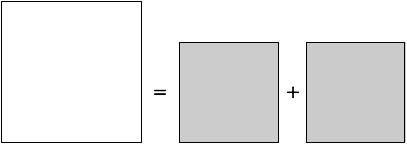
\includegraphics[scale=0.4]{FiguresArithmetic/sqrt2initial}
\caption{{\it A geometric depiction the Pythagorean Theorem and its
    underlying equation: $a^2 = b^2 + b^2$.}
\label{fig:irrationality1}}
\end{center}
\end{figure}
suggestively invokes the Pythagorean Theorem.  The figure presents
three squares.  The intention is that the two small grey squares are
identical, with common area $A$, while the large white square has
double this area.  By the Pythagorean Theorem, if the small squares
have (common) side-lengths $b \in \N^+$, hence shared area $A = b^2$,
then the large square has side-lengths $a \eqdef \sqrt{2}b$, hence
area $a^2 = 2 b^2$.

Thus set up, we begin to pursue our contradiction.  As in the
classical proof in Section~\ref{sec:classical-proof-sqrt(2)}, we start
with the assumption that $\sqrt{2}$ is rational.  Within the context
of Fig.~\ref{fig:irrationality1}, this means that
\[ \sqrt{2} \ = \ {a \over b} \]
for $a, b \in \N^+$.  Since all that we have said thus far holds for
arbitrary $a$ and $b$, we are free to consider the assumption's
implications for the same situation as in
Section~\ref{sec:classical-proof-sqrt(2)}, namely, that $a$ and $b$ do
not share any common prime factor.  Note additionally that,
because\footnote{If this inequality is new to you, then just note that
  $(1.4)^2 = 1.96$, which is less than $2$.}
\[ \sqrt{2} \ > \ 1.4, \]
we know that $a > b$.

\[ \approx \approx \approx \approx \approx \approx \approx \approx \approx \approx \]
Of course, our demands on the relationship between the numerator $a$
and the denominator $b$ lose no generality in our argument.  To wit,
``$\displaystyle {a \over b}$'' is just one name for the depicted
rational number, and choosing any specific name has no impact on the
number itself.
\[ \approx \approx \approx \approx \approx \approx \approx \approx \approx \approx \]

Now that we have the suggestive ``equation'' presented in
Fig.~\ref{fig:irrationality1}, we can manipulate the depicted squares.
Let us embed both of the grey $b \times b$ squares of
Fig.~\ref{fig:irrationality1} into the white $a \times a$ square, in
the overlapped manner depicted in Fig.~\ref{fig:irrationality2}:
\begin{figure}[htb]
\begin{center}
       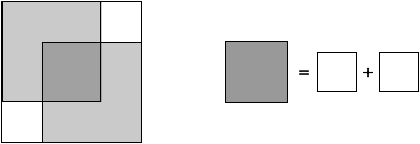
\includegraphics[scale=0.4]{FiguresArithmetic/sqrt2final}
\caption{{\it Construction of a smaller pythagorian equation.}
\label{fig:irrationality2}}
\end{center}
\end{figure}
one grey square is nestled into the northwestern corner of the white
square, while the other is nestled into the southeastern corner.
The overlapping of the grey squares under this
embedding creates a new square---depicted in dark grey---in the center
of the white square, while it leaves unoccupied two small squares,
which remain white in the figure.

Now, let us get quantitative.
\begin{enumerate}
\item
The fact that the combined areas of the two grey squares equals the
area of the white square guarantees that the area of the dark grey
overlap-square is equal to the combined areas of the small unoccupied
white squares.

\item
Because the side-lengths of the large white square is $a$, while those
of the grey squares is $b$, the side-lengths of the small white square
is $a-b$, and the side-lengths of the dark grey overlap-square is
$2b-a$.  All of these side-lengths are positive because of the value
of $\sqrt{2}$: ($i$) $a > b$ because $\sqrt{2} >1$; ($ii$) $2b >a$
because $\sqrt{2} < 2$.
\end{enumerate}
The preceding facts allow us to label the squares of
Fig.~\ref{fig:irrationality1} differently than we did earlier---and
derive a different valid ``equation''.  As we did at the beginning of
this discussion, we again invoke the Pythagorian Theorem, but now we
do so while focusing---cf., Fig.~\ref{fig:irrationality2}---on the
dark grey overlap-square (which plays the role of the large square in
Fig.~\ref{fig:irrationality1}) and the two small white squares (which
play the role of the two small squares in
Fig.~\ref{fig:irrationality1}).  Whereas our original focus led to the
putative rational value $\displaystyle {a \over b}$ for $\sqrt{2}$,
the new focus yields the putative rational value $\displaystyle {2b-a
  \over a-b}$ for $\sqrt{2}$.  We thus have
\[ \sqrt{2} \ = \ {a \over b} \ = \ {2b-a \over a-b}, \]
where $2b-a < a$ and $a-b < b$.  In the light of the Fundamental
Theorem of Arithmetic (Theorem~\ref{thm:Fund-Thm-Arith}), this new
rational name for $\sqrt{2}$ contradicts our beginning assumption that
$\displaystyle {a \over b}$ is the simplest name.
\qed
\end{proof}

\subsection{$\R$ is uncountable, hence is ``bigger than'' $\Z$ and $\Q$}
\label{sec:Q-Z-R-cardinality}
\label{sec:Reals-uncountable}

\ignore{\Arny Do we want to include the diagonal argument.  It is beautiful --- but is it ``core''?}
\ignore{\Denis yes, I think so}

The main result of this section establishes the uncountability of the
set $\R$.  We thereby have an argument that the infinitude of real
numbers is {\em of a higher order} than the infinitude of the
integers.  In fact, Georg Cantor used this result as the base of
his study of orders of infinity.

\begin{prop}
\label{thm:R-uncountable}
The set $\R$ of real numbers is not countable.
In particular, there is no injection $f: \R \rightarrow \N$.
\end{prop}

\begin{proof}
Our multi-step proof shows that the assumption of $\R$'s countability
leads to a contradiction.  Being built around Georg Cantor's renowned
{\it diagonalization construction}, \index{diagonalization} this
argument provides the most sophisticated proof by contradiction in our
text.  The reader might want to review the reasoning underlying such
argumentation, in Chapter~\ref{sec:Contradiction}, as a ``warm-up.''

\subsubsection{Plotting a strategy to prove uncountability}

Invoking the definition of countability, our proof begins with the
assumption that $|\R| \leq |\N|$ and demonstrates that this assumption
leads to a contradiction.  We simplify our goal in several steps.

{\it (a) Recasting the problem in terms of bijections.}
We now set out to recast our goal into a form that will be easier to
manage mathematically, by invoking our prior knowledge about the sets
$\N$ and $\R$.  We begin with two simplifying lemmas.

\begin{lemma}
\label{lem:N-leq-R}
There exists an injection $f: \N \rightarrow \R$; i.e., $|\N| \leq
|\R|$.
\end{lemma}

\noindent {\it Verification}.
%
For each nonnegative integer $n \in \N$, let $\mbox{\sc num}_b(n)$
denote the shortest base-$b$ numeral for $n$, i.e., a numeral with no
leading $0$s.  The mapping that associates each $n \in \N$ with the
infinite string
\[ \mbox{\sc num}_b(n) \ . \ 00 \cdots \]
is an injection from $\N$ into $\R$.  To wit, when given a real
numeral that has only $0$s to the right of its radix point, one
produces the integer $n$ by stripping the numeral of its radix point
and all $0$s to the right of the point, and then evaluating the
remaining string of digits, which is $\mbox{\sc num}_b(n)$, according
to Section~\ref{sec:define-Reals}'s rules for evaluating integer
numerals.  \qed

\begin{lemma}
\label{lem:N-=-R}
If there exists an injection $g: \R \rightarrow \N$, then there exists
a bijection $h: \N \leftrightarrow \R$.  In other words, if $|\R| \leq
|\N|$, then $|\N| = |\R|$.
\end{lemma}

\noindent {\it Verification}.
This is an immediate consequence of the Schr\"{o}der-Bernstein Theorem
(Theorem~\ref{thm.S-B}).  \qed

\medskip

It is somewhat surprising that our proof is simplified by converting
our initial assumption \\
\hspace*{.35in}$|\R| \leq |\N|$ \\
to the stronger assumption \\
\hspace*{.35in}$|\R| \ = \ |\N|$,  \\
but Cantor's diagonal argument deals quite gracefully with the latter
assumption.

\medskip

{\it (b) Focus on real numbers between $0$ and $1$.}
Our next refinement replaces our target set $\R$ by its proper subset
$\R_{(0,1)}$, all of whose elements have infinite decimal numerals of
the form
\[ 0 \ . \ \delta_0 \delta_1 \cdots \]
where each $\delta_i$ is a decimal digit: $\delta_i \in \{0, 1, 2, 3,
4, 5, 6, 7, 8, 9\}$.\footnote{We choose {\em decimal} numerals for
  convenience: converting the argument to other number
  bases---especially the base $b=2$---slightly complicates clerical
  details.}

Of course, if we prove that the proper subset $\R_{(0,1)} \subset \R$
is uncountable, then it will follow that $\R$ is uncountable.  (In
informal terms which can be made formal, any putative injection $f: \R
\rightarrow \N$ ``contains'' an injection $f_{(0,1)}: \R_{(0,1)}
\rightarrow \N$.)

\subsubsection{Seeking a bijection $h: \N \leftrightarrow \R_{(0,1)}$}

We assume, for contradiction, that the targeted bijection $g$ exists.
As part of this two-way mapping, there exists an {\em injection}
\[ 
h: \N \ \rightarrow \ \R_{(0,1)},
\]
which we view as an {\em enumeration} of the elements of $\R_{(0,1)}$.
Specifically, for each integer $k \in \N$, we can think of $h(k)$ as
the ``$k$th number in the set $\R_{(0,1)}$.''  We thereby view $h$ as
producing an ``infinite-by-infinite'' matrix $\Delta$ of decimal
digits, whose $k$th row is the infinite string of decimal digits
$\mbox{\sc num}_{10}(h(k))$.  Let us visualize $\Delta$:
\[ \Delta \ = \
\begin{array}{ccccccc}
\delta_0 = &
\delta_{0,0} & \delta_{0,1} & \delta_{0,2} & \delta_{0,3} &
	\delta_{0,4} & \cdots \\
\delta_1 = &
\delta_{1,0} & \delta_{1,1} & \delta_{1,2} & \delta_{1,3} &
	\delta_{1,4} & \cdots \\
\delta_2 = &
\delta_{2,0} & \delta_{2,1} & \delta_{2,2} & \delta_{2,3} &
	\delta_{2,4} & \cdots \\
\delta_3 = &
\delta_{3,0} & \delta_{3,1} & \delta_{3,2} & \delta_{3,3} &
	\delta_{3,4} & \cdots \\ 
\delta_4 = &
\delta_{4,0} & \delta_{4,1} & \delta_{4,2} & \delta_{4,3} &
	\delta_{4,4} & \cdots \\ 
\vdots &
\vdots  & \vdots  & \vdots  & \vdots  & \vdots  & \ddots
\end{array}
\]

\noindent We summarize, for emphasis:
\begin{itemize}
\item
Each row of $\Delta$ consists of the decimal numeral for a number in
the set $\R_{(0,1)}$.

\item
Each number in the set $\R_{(0,1)}$ contributes at least one numeral
to the rows of $\Delta$.

A number may contribute more than one numeral because of an artifact
of positional number systems, which is exemplified by equations such
as
\[ 0.25 \ = \ 0.24999\cdots \]
\end{itemize}
We can, thus, view the successive rows of $\Delta$, $h(0)$, $h(1)$,
\ldots, as an enumeration (with possible repetitions) of all of the
real numbers in the set $\R_{(0,1)}$.

\subsubsection{Every proposed bijection $h: \N \leftrightarrow \R$
  ``misses'' some $x \in \R_{(0,1)}$}

We are finally poised to find the contradiction to our assumption that
$|\R_{(0,1)}| \leq |\N|$.  Specifically, we define from $\Delta$ an
infinite decimal numeral
\[ \Psi \ = \ \psi_0 \ \psi_1 \ \psi_2 \ \psi_3 \ \psi_4 \cdots, \]
that {\em does not} appear in $\Delta$, even though $\mbox{\sc
  num}_{10}(\Psi) \in \R_{(0,1)}$.  For each index $i \in \N$, we
define the $i$th digit $\psi_i$ of $\Psi$ from the $i$th {\em diagonal
  digit}\footnote{Our use of $\Delta$'s ``diagonal digits'' in this
  definition is the origin of the term ``{\em diagonal argument}'' to
  describe this proof and its intellectual kin.}~$\delta_{i,i}$ of
$\Delta$ in the following manner.
\[ \psi_i \ \eqdef \
%= \ \overline{\delta}_{i,i} \ \eqdef \
\left\{
\begin{array}{cc}
0 & \mbox{ if } \ \delta_{i,i} \ > \ 5 \\
9 & \mbox{ if } \ \delta_{i,i} \ \leq \ 5 \\
\end{array}
\right.
\]
The important feature of the definition is the following.

\begin{lemma}
\label{lem:PSI-notin-DELTA}
The string $\Psi$ does not occur as a row of $\Delta$.
\end{lemma}

\noindent {\it Verification}.
Focus on an arbitrary row of $\Delta$, say row $k$, and on the numeral,
$\delta_k$, in that row.

\begin{tabular}{lclc}
If & $\delta_{k,k} \ > \ 5$ & then & \ \
$\mbox{\sc num}_{10}(\delta_k) \ - \ \mbox{\sc num}_{10}(\Psi) \ > \ 4
\cdot 10^{-k}$ \\
If & $\delta_{k,k} \ \leq \ 5$ & then & \ \
$\mbox{\sc num}_{10}(\Psi) \ - \ \mbox{\sc num}_{10}(\delta_k) \ > \ 4
\cdot 10^{-k}$
\end{tabular}

\noindent
In either case, we have $\mbox{\sc num}_{10}(\Psi) \ \neq \ \mbox{\sc
  num}_{10}(\delta_k)$ so that $\Psi$ does not appear as row $k$ of
$\Delta$.  Since $k \in \N$ is an arbitrary row-index of $\Delta$, we
conclude that $\Psi$ does not occur as any row of $\Delta$.  \qed

\subsubsection{The denouement: There is no bijection  $h: \N \leftrightarrow \R$}

Because the infinite decimal string $\Psi$ differs from every row of
$\Delta$, even though $\mbox{\sc num}_{10}(\Psi) \in \R_{10}$, we have
shown that $\Delta$ {\em does not} contain as a row {\em every}
infinite decimal numeral of a number in $\R_{10}$.  But this
contradicts $\Delta$'s assumed defining characteristic!

Where could we have gone wrong?  Every step of our argument, save one,
is backed up by a proof---so the one step that is not so bolstered
must be the link that has broken.  This one unsubstantiated step is
our assumption that the set $\R_{10}$ is countable.  Since this
assumption has led us to a contradiction, we must conclude that the
set $\R_{10}$, and hence, the set $\R$, is {\em not} countable!
\qed
\end{proof}



\section{The Complex Numbers}
\label{sec:complexes}


\subsection{The Basics of the Complex Numbers}

$\C$ denotes the complex numbers

Each complex number $\kappa = a+bi \in \C$ has a {\it real part}---the
part that {\em does not} involve the imaginary unit $i$---and an {\it
  imaginary part}---the part that {\em does} involve $i$.  To be
explicit: the real part of our number $\kappa$, is Re$(\kappa) = a$;
\index{complex number!real part Re($\cdot$)}
the {\it imaginary part} of our number $\kappa$,is Im$(\kappa) = b$.
\index{complex number!imaginary part Im($\cdot$)}
The notation Re$(\kappa)$ and Im$(\kappa)$ is common but not
universal.

\index{complex number!multiplication!three real multiplications}
Using the basic arithmetic laws that we have discussed thus far, plus
the defining equation, $i^2 = -1$, of the imaginary unit $i$, we find
that the {\em product} of two complex numbers, $a+bi \in \C$ and $c+di
\in \C$ is the complex number, call it $\kappa$,
\begin{equation}
\label{eq:complex-mult}
\kappa \ = \ (a+bi) \cdot (c+di) \ = \ (ac - bd) + (ad + bc)i.
\end{equation}
We note that a ``direct'' implementation of complex multiplication,
i.e., one that implements (\ref{eq:complex-mult}) literally, requires
four real multiplications---namely, $ac, bd, ad, bc$.

During the 1960s, people first began to pay close attention to the
costs associated with various ways of achieving computational results.
They sought---and found---a number of procedures that replaced
computations involving $k$ real multiplications (a relatively
expensive operation) and $\ell$ real additions (a relatively
inexpensive operation) by computations that achieved the same result
but used fewer multiplications and not too many more additions.
Complex multiplication was one of the operations they studied.  Here
is the result.

\addcontentsline{toc}{paragraph}{-- A fun result: complex
  multiplication via $3$ real multiplications}
\index{complex number!multiplication via 3 real multiplications}

\begin{prop}
\label{thm:complex-mult-3real}
One can compute the product of two complex numbers using {\em three}
real multiplications rather than four.
\end{prop}

\begin{proof}
Although implementing (\ref{eq:complex-mult}) ``directly'' correctly
produces the product $\kappa = (a+bi) \cdot (c+di)$, there is another
implementation that is {\em more efficient}.  Specifically, the
following recipe computes $\kappa$ using only {\em three} real
multiplications instead of the four real multiplications of the
``direct'' implementation.  We begin to search for this recipe by
noting that our immediate goal is to compute both Re$(\kappa) = ac-bd$
and Im$(\kappa) = ad+bc$.  We can accomplish this by computing the
{\em three} real products
\begin{equation}
\label{eq:complex-mult-3a}
(a+b) \cdot (c+d); \ \ \ \ \
ac;  \ \ \ \ \ bd
\end{equation}
and then noting that
\begin{equation}
\label{eq:complex-mult-3b}
\begin{array}{lcl}
\mbox{Re}(\kappa) & = & (a+b) \cdot (c+d) - ac -bd, \\
\mbox{Im}(\kappa) & = & ac -bd
\end{array}
\end{equation}
We thereby achieve the result of the complex multiplication described
in (\ref{eq:complex-mult}) while using only {\em three} real
multiplications.

Of course, a full reckoning of the costs of the two implementations we
have discussed exposes the fact that the implementation that invokes
(\ref{eq:complex-mult-3a}) and (\ref{eq:complex-mult-3b}) uses {\em
  three} real additions rather than the {\em two} real additions of
the ``direct'' implementation.  But this entire exercise was
predicated on the observation that each real addition is much less
costly than a real multiplication, so trading one multiplication for
one addition is an unqualified ``win''.  \qed
\end{proof}


\section{Finite Number Systems}
\label{sec:congruences+modular}

The sets that underlie the number systems that we use in most daily
tasks---namely $\N, \Z, \Q$, and $\C$---are infinite: we can always
find a number in each set that is bigger than all the numbers we have
seen thus far.  Indeed, the last two of these sets are ``two-way''
infinite: we can also always find a number in each set that is smaller
than all the numbers we have seen thus
far.\footnote{\label{foot:Pascal}The philosophically inclined reader
might be interested in the essay ``The Two Infinities'' within the
{\it Pens\'{e}es} of the French mathematician-philosopher (or
philosopher-mathematician?) Blaise Pascal \index{Pascal, Blaise},
whose work we shall revisit in Chapter~\ref{sec:binary-operators}.C.}
There do, however, exist several very important situations in which we
use number systems that are {\em finite} and {\em cyclically
  repetitive}.  We mention only two.
\begin{itemize}
\item
The {\em clocks} that we use to indicate daily time are calibrated
into a fixed finite number of major subdivisions, {\em hours}.  We
endow our days with $24$ hours and depending on circumstances, have
our clocks measure each day's time via repeating cycles of either $12$
or $24$ hours.  Once a clock's limit of ($12$ or $24$ hours) has been
reached, it begins its numeration all over---with no memory of the
past.

\item
We typically orient all manner of location specification relative to a
fixed reference point in terms of {\em angles}.  There are two
coexisting, competing systems for such measurement.  One system
subdivides the ``circle'' around the reference point into $360$ {\em
  degrees;} the other subdivides the ``circle'' into $2 \pi$ {\em
  radians}.  For our purposes, the main interesting point is that both
of these systems are {\em cyclically repetitive}.  Once we have
circled the reference point by $360$ degrees (or, equivalently, by $2
\pi$ radians), then we measure further circumnavigation starting over
at $0$ degrees/radians.
\end{itemize}

This section is dedicated to integer-based {\em finite} number systems
that were invented to describe and measure cyclically repetitive
situations such as the two just described.


\subsection{Congruences on Nonnegative Integers}
\label{sec:congruences}

For any positive integer $q \in \N^+$, we denote by $\N_q$ the
$q$-element ``prefix'' of the set $\N$ of nonnegative integers:
\index{$\N_q$: the first $q$ nonnegative integers}
\[ \N_q \ \eqdef \ \{0, 1, \ldots, q-1\} . \]
For nonnegative integers $m, n \in \N$ and positive integer $a \in
\N^+$, we say that {\em $m$ is congruent to $n$ modulo $q$},
\index{integer congruence} \index{congruent to} denoted
\[ m \equiv n \bmod q, \]
precisely when $q \mbox{ divides } |m-n|$.  We call $q$ the {\it
  modulus} of the congruence (relation).
\index{modulus}

\begin{prop}
\label{thm:CONGisEQUIVALENCE-REL}
The relation of congruence modulo a positive integer is an equivalence
relation on the set $\N$ of nonnegative integers.
\end{prop}

\begin{proof}
We verify in turn the three defining properties of an equivalence
relation (see Chapter~\ref{sec:equiv-relation}).  Focus on nonnegative
integers $m$, $n$, and $r$ and an arbitrary positive integer modulus
$q$.

\begin{enumerate}
\item
Congruence modulo $q \in \N^+$ is a {\em symmetric} relation on $\N$.

{\it Verification:}
Because $|m-n| = |n-m|$, the assertions $[q \mbox{ divides } |n-m|]$
and $[q \mbox{ divides } |n-m|]$ must hold simultaneously, i.e.,
either both assertions are true or neither is.

\item
Congruence modulo $q \in \N^+$ is a {\em reflexive} relation on $\N$.

{\it Verification:}
We always have $m \equiv m \bmod q$ because every positive integer
divides $m-m = 0$.

\item
Congruence modulo $q \in \N^+$ is a {\em transitive} relation on $\N$.

{\it Verification:}
Say that $m \equiv n \bmod q$ and $n \equiv r \bmod q$.  The
arithmetic needed to verify that these two congruences imply that $m
\equiv r \bmod q$ breaks down into cases defined by the relative sizes
of $m$, $n$, and $r$.  We supply the details for the case $m > n > r$,
and we leave the other cases as exercises.

Note first that the two assumed conguences can be rewritten as
assertions of divisibility: $q \mbox{ divides } |m-n|$, and $q \mbox{
  divides } |n-r|$.  Therefore, in the chosen case $m > n > $, the
congruences imply that there exist integers $c_1$ and $c_2$ such that:
  \begin{enumerate}
  \item
$c_1 q = m-n$, which implies that $n = m - c_1 q$;
  \item
$c_2 q = n-q$, which implies that $n = q + c_2 q$.
  \end{enumerate}
We therefore have $r-m = (c2-c_1) q$, which means that $m \equiv r
\bmod q$.  In other words, The relation $equiv \bmod q$ is transitive.
\end{enumerate}
The preceding three properties define an equivalence relation, hence,
jointly verify the proposition.
\qed
\end{proof}

\subsection{Finite Number Systems via Modular Arithmetic}
\label{sec:modular}

Once we embellish the sets $\N_q$ with arithmetic operations---namely,
the ``big four'' of addition, subtraction, multiplication, and
division---we shall see why we are able to use the resulting
congruential systems in the same way as their infinite counterparts,
$\N$, $\Z$, and $\Q$.  In the coming subsections, we show that every
set $\N_q$ can ``mimic'' $\N$ and $\Z$ with respect to addition,
subtraction, and multipliciation, but only when $q$ is a prime number
can $\N_q$ ``mimic'' $\Q$ with respect to division.

\subsubsection{Sums, differences, and products exist within $\N_q$}
\label{sec:modular-add-sub-mult}

Our main result in this section demonstrates that every set $\N_q$,
when embellished with the operations addition, subtraction, and
multiplication, is {\em closed}\index{algebraic closure}\index{closure
  under an arithmetic operation} under these operations, in the sense
spelled out in the following result.

\begin{prop}
\label{thm:modular-add-sub-mult}
For every integer $q \in \N^+$ and all $m,n \in \N_q$, the sum $m+n
\bmod q$ and the difference $m-n \bmod q$ and the product $m \cdot n \bmod
q$ exist within $\N_q$.
\end{prop}

\begin{proof}
For the operations of addition and multiplication, the result is true
by definition of congruence modulo $q$: since the sum $m+n$ and the
product $m \cdot n$ exist within $\N^+$, their ``reductions'' modulo
$q$ exist within $\N_q$.  For the case of subtraction, we augment the
preceding sentence with the following equation.  For all $r \in \Z$
\[ q-r \ \equiv \ -r \bmod q. \]
One verifies this equation by noting the following chain of equalities
and congruences (parentheses added to enhance legibility)
\[ (q-r) - (-r) \ \ = \ \ (q-r) + r \ \ = \ \ q \ \ \equiv \ 0 \bmod q. \] 
In all cases, therefore, the result of the operation remains in the set
$\N_q$.
\qed
\end{proof}

We cannot generally add division to the set of operations listed in
Proposition~\ref{thm:modular-add-sub-mult}.  For instance, the
following table shows that the equation 
\[ 2x \ \equiv \ 1 \bmod 6 \]
is not solvable for all $x \in \N_6 \setminus \{0\}$.
\[ \begin{array}{|c|c|}
\hline
x & 2 \cdot x \bmod 6 \\
\hline
\hline
1 & 2 \\
2 & 4 \\
3 & 0 \\
4 & 2 \\
5 & 4 \\
\hline
\end{array}
\]
The next subsection implicitly identifies the modulus $6$'s
non-primality as the culprit in this example.  In fact, the reader can
easily show that {\em $\N_q$ is never closed under the operation of
  division when the modulus $q$ is composite, i.e., nonprime.}


\subsubsection{Quotients exist within $\N_p$ for every prime $p$}
\label{sec:modular-quotientss}

This section considers congruences modulo a prime number.  We begin
with our main result: {\em for every prime number $p$, every nonzero
  $n \in \N_p$ has a {\em multiplicative inverse}}, i.e., an element
$m \in \N_p$ such that $m \cdot n \equiv 1 \bmod
p$. \index{multiplicative inverse} Of course, the existence of
multiplicative inverses allows one to {\em divide} any number in
$\N_p$ by any nonzero number.

\begin{prop}
\label{thm:finite-field}
For every prime number $p$, every nonzero number $n \in \N_p$ has a
multiplicative inverse within $\N_p$.
\end{prop}

\begin{proof}
Our proof combines applications of the Fundamental Theorem of
Arithmetic (Theorem~\ref{thm:Fund-Thm-Arith}) and the Pigeonhole
Principle (Section~\ref{sec:pigeonhole}), alongside a proof by
contradiction.  It thereby exercises many of our important new proof
techniques.

Focus on the set $\N_p$ for some prime $p$.  Let $n$ be any nonzero
number in $\N_p$.  

\begin{lemma}
\label{lem:multiples-in-Zp-unique}
There do {\em not} exist nonzero numbers $m_1$ and $m_2 \neq m_1$ in
$\N_p$ such that $m_1 \cdot n \equiv m_2 \cdot n \bmod p$.
\end{lemma}

\begin{proof} ({\em of Lemma~\ref{lem:multiples-in-Zp-unique}})
Assume for contradiction that there {\em do} exist $m_1$ and $m_2 \neq
m_1$ in $\N_p$ such that $m_1 \cdot n \equiv m_2 \cdot n \bmod p$.
Say, with no loss of generality, that $m_1 > m_2$ within the set $\N$.
We must then have
\begin{equation}
\label{eq:a-forbidden-divisibility}
p \ \mbox{ divides } \ (m_1 - m_2) \cdot n.
\end{equation}
The fact that $p$ is a prime ensures---by
Proposition~\ref{thm:p-divides-onefactor}---that $p$ divides at least
one of the integers $n$ or $(m_1 - m_2)$.  Because both of these
integers belong to $\N_p$, hence lie strictly between $0$ and $p-1$
(within the infinite set $\N$), the divisibility posited in
(\ref{eq:a-forbidden-divisibility}) is impossible!  The lemma follows.
\qed
\end{proof}

Lemma~\ref{lem:multiples-in-Zp-unique} guarantees that all of the
following $p-1$ elements of $\N_p$ are nonzero and distinct:
\[ 1 \cdot n, \ \ 2 \cdot n, \ldots, \ \ (p-1) \cdot n. \]
Because $\N_p$ has precisely $p-1$ nonzero elements, these $p-1$
multiples of $n$ must exhaust these elements.  In other words, some
multiple of $n$, say $c \cdot n$, must equal $1$.  This means that the
number $c \in \N_p$ is $n$'s multiplicative inverse within $\N_p$.
\qed
\end{proof}

\medskip

Of course, once we have multiplicative inverses, we have the operation
of division and, consequently, arbitrary quotients and fractions.  Of
course, fractions within finite number systems such as $\N_p$ are
going to look strange to our eyes, as the following example indicates.

What does the number $7/4$ look like within $\N_5$?  We develop the
answer in steps.

\[ \approx \approx \approx \approx \approx \approx \approx \approx \approx \approx \]
We are able to proceed in the following manner because the relations
($\equiv \bmod q$) are {\em congruences}, \index{congruence relation}
i.e., equivalence relations whose class structures are consistent with
the algebraic structure of the arithmetic systems exemplified by $\Z$,
$\Q$, $\R$, and $\N_p$ under the classical four arithmetic operations.
A full treatment of this topic is beyond the scope of this text.
\[ \approx \approx \approx \approx \approx \approx \approx \approx \approx \approx \]
\begin{enumerate}
\item
The numbers $4, 7 \in \N$ correspond, respectively, to the numbers $4,
2 \in \N_5$.

Verification:
$4 \equiv 4 \bmod 5$, and $7 \equiv 2 \bmod 5$.

\item
The multiplicative inverse of $4$ within $\N_5$ is $4$.

Verification:
$4 \cdot 4 \ = \ 16 \ \equiv 1 \bmod 5$.

\item
THEREFORE, we have the following ``translation'' of the quotient $7/4$:

Within $\N$: \\
the product of $7 \in \N$ by the multiplicative inverse of $4 \in \N$

Within $\N_5$: \\
the product of $2 \in \N_5$ by the multiplicative inverse of $4 \in
\N_5$, which is $4$

\item
the product of $2 \in \N_5$ by $4 \in \N_5$ is $3$.

Verification:
$2 \cdot 4 \ = \ 8 \ \equiv 3 \bmod 5$.
\end{enumerate}
We thus have the unintuitive fact that the rational number $7/4$
corresponds to the number $3 \in \N_6$.

Of course, we do not often perform arbitrary arithmetic within the
finite number systems $\N_p$, so we do not often struggle with the
unfamiliar results of this subsection.  That said, we do sometimes
intermix ``ordinary'' numeration with ``modular'' numeration, as when
we coordinate talk about elapsed time (measured in the ``ordinary''
way) with wall-clock time (which is a ``modular'' system).  So, in
summation, it is worth the effort to understand this seldom-used
material.  Plus, it can be amusing to announce at a party that you can
``prove'' that $1.75 = 3$.


\section{Numerals We Can Work With}\index{numerals}
\label{sec:Numerals}


\subsection{Positional Number Systems}
\label{sec:positional-numbers}
\index{positional number system}

The most common family of {\em operational}
\index{numerals!operational} numerals for real numbers---i.e.,
numerals that enable one to do things such as perform arithmetic (add,
multiply, etc.) on the named numbers---is the family of {\it
  positional number systems}.  Each system in this family is
identified by its {\em base}, 
\index{positional number system!base}
which is usually\footnote{In rather specialized contexts one
  encounters number bases that are not positive integers.}~an
integer $b >1$.
\index{positional number system!base-$b$ numeral}
For any base $b$, we define the set $B_b = \{ 0, 1, \ldots, b-1\}$ of
{\it digits in base $b$}.\index{positional number system!digits in
  base $b$}
%
To aid legibility, {\em within the context of base-$b$ positional
  numerals}, we denote the digit $b-1$ as a single character, $\bar{b}$.
\index{$\bar{b}$: the digit $b-1$ in base $b$}
%
We then form base-$b$ numerals in the following way.
\index{positional number system!base-$b$ numerals}
\[ \approx \approx \approx \approx \approx \approx \approx \approx \approx \approx \]
{\em The entire edifice of positional numerals builds on the concept
  of {\em geometric summations}, a mathematical structure that we
  shall learn to manipulate, evaluate, and compute with in
  Section~\ref{sec:geometric-sums}.  We need only special aspents of
  this topic here.
}
\[ \approx \approx \approx \approx \approx \approx \approx \approx \approx \approx \]

A base-$b$ numeral is a string having three segments.
\begin{enumerate}
\item
The numeral begins with its {\em integer part},
\index{positional number system!integer part of a numeral}
%
which is a {\em finite} string of digits from $B_b$.  We denote the
integer-part string as: $\alpha_n \alpha_{n-1} \cdots \alpha_1
\alpha_0$.

\item
The numeral continues with a single occurrence of the {\it
  radix point}\index{positional number system!radix point ``$.$''}
``$.$''

\item
The numeral ends with its {\em fractional part},\index{positional
  number system!fractional part of a numeral}
%
which is a string---{\em finite or infinite}--- of digits from $B_b$.
We denote the fractional-part string as:
$\beta_0 \beta_1 \beta_2 \cdots$.
\end{enumerate}
Our completed numeral now has the form
\begin{equation}
\label{eq:real-numeral}
\alpha_n \alpha_{n-1} \cdots \alpha_1 \alpha_0
\ . \ \beta_0 \beta_1 \beta_2 \cdots
\end{equation}
where the $\alpha_i$ and the $\beta_j$
\index{positional number system!base-$b$ digits} 
are {\em base-$b$ digits} i.e., elements of the set $B_b$, and
``$.$'' represents the {\em (base-$b$) radix point}.

\noindent
The numeral depicted in (\ref{eq:real-numeral}) represents the (real)
number\footnote{The notation ``$\mbox{\sc value}(x)$'' in
  (\ref{eq:real-numeral-number}) denotes an operator that produces the
  {\em numerical value} of the numeral $x$.}
\begin{equation}
\label{eq:real-numeral-number}
\mbox{\sc value}(\alpha_n \alpha_{n-1} \cdots \alpha_1 \alpha_0                  
\ . \ \beta_0 \beta_1 \beta_2 \cdots)
\ \ \eqdef \ \
\sum_{i=0}^n \alpha_i \cdot b^i
\ + \ \sum_{j\geq 0} \beta_j \cdot b^{-j}.
\end{equation}
\index{positional number system!numerical value of numeral}

For emphasis, we note that the base-$b$ integer 
\index{positional number system!numerical value of integral part}
represented by the numeral's integer part is
\[
\mbox{\sc value}(\alpha_n \alpha_{n-1}\cdots \alpha_1 \alpha_0)
\ \ = \ \
\sum_{i=0}^n \alpha_i \cdot b^i
\]
and the base-$b$ fraction represented by the numeral's fractional part
is\index{positional number system!numerical value of fractional part}
\[
\mbox{\sc value}(. \beta_0 \beta_1 \beta_2 \cdots)
\ \ = \ \
\sum_{j\geq 0} \beta_j \cdot b^{-j}
\]
By prepending a ``minus sign'' (or, ``negative sign'') $-$ to a
numeral or a number, one renders the thus-embellished entity as
negative.

\medskip

Note that {\em two types of sequences of $0$s do not affect the value
  of the number represented by a numeral:} (1) an {\em initial}
sequence of $0$s to the {\em left} of the radix point and of all
non-$0$ digits; (2) a {\em terminal} sequence of $0$s to the {\em
  right} of the radix point and of all non-$0$ digits.

One consequence of this fact is that we lose no generality by
insisting that every numeral have the following {\em normal form:}
\index{positional number system!numeral!normal form}
\index{normal form for for numeral in a positional number system}

\smallskip

\hspace*{.15in}
\begin{tabular}{l}
-- a finite sequence of digits, \\
-- followed by a radix point, \\
-- followed by an infinite sequence of digits
\end{tabular}


\subsection{Recognizing Integers and  Rationals from Their Numerals}
\label{sec:special-numerals-N-Q}

We have provided an adequate, albeit inelegant, characterization of
the real numbers: a number $r$ is real if,and only if, it can be
represented by an infinite-length numeral in a positional number
system.  Because every rational number---hence, also, every
integer---is also a real number, every rational number and every
integer can also be written as a$b$-ary numeral, in the form
(\ref{eq:real-numeral}).  For rational numbers and integers, we can
make much stronger statements about the forms of their positional
numerals.

\subsubsection{Positional numerals for integers}
\label{sec:special-numerals-N}

\begin{prop}
\label{thm:integer-real}
A real number is an integer if, and only if, it can be represented by
a {\em finite-length} numeral all of whose nonzero digits are to the
left of the radix point.
\index{number!integer!real with a finite numeral}
\end{prop}

\begin{proof}
The result is immediate by definition (\ref{eq:real-numeral-number}).
In the indicated form, if any $\beta_i$ is nonzero, then the {\sc
value} of the numeral is non-integral: it has a nonzero fractional part.
\qed
\end{proof}

We can go beyond the simple statement of
Proposition~\ref{thm:integer-real} and present the following algorithm
that computes the normal-form base-$b$ numeral for an integer $n$.

\bigskip

\noindent {\underline{\bf Procedure}} {\small\sf Normal-Form
  Numeral}($n$)

/*Compute the normal-form numeral for a given integer $n$*/

\smallskip

\noindent{\bf Initialization}.

Set {\sc current-residue} to $n$

\smallskip

\noindent{\bf Iteration}. 

Until {\sc current-residue} $= 1$

Divide {\sc current-residue} by $b$

\medskip

\noindent
The {\em remainder} upon each division is the next lowest-order
digit in the base-$b$ numeral for $n$.


\bigskip

\noindent {\it Validating the procedure.}
%
The procedure is an implementation of a method of rewriting univariate
polynomials, known variously as {\it Horner's rule} or {\it Horner's
  scheme} \cite{Horner}.  
\index{Horner's rule} \index{Horner's scheme}
Among its other virtues, the ``rule'' provides a recipe for computing
a degree-$d$ univariate polynomial using $O(d)$ multiplications,
rather than the $\Theta(d^2)$ multiplications that appear at first to
be needed.

\medskip

\noindent {\small\sf The ``standard'' way of writing the polynomial $P(x)$.}

\noindent General degree $d$:

$P(x) \ \ = \ \ a_0 \ + \ a_1 x \ + \ a_2 x^2 \ + \cdots + \ a_{d-1}
x^{d-1} \ + \ a_d x^d$

\noindent Degree $3$:

$P(x) \ \ = \ \ a_0 \ + \ a_1 x \ + \ a_2 x^2 \ + \ a_3 x^3$

\medskip

\noindent {\small\sf Rewriting $P(x)$ using Horner's rule.}

\noindent General degree $d$:

$P(x) \ \ = \ \ a_0 \ + \ x \cdot (a_1 \ + \ x \cdot (a_2  \ +  \cdots
+ x \cdot (a_{d-2} \ + \ x \cdot (a_{d-1} \ + \ a_d x)) \cdots ))$  

\noindent Degree $3$:

$P(x) \ \ = \ \ a_0 \ + \ x \cdot (a_1 \ + \ x \cdot (a_2  \ + \ a_3 x))$ 

\medskip

The ``rule'' is so natural that its origins certainly predate the
cited 1819 publication, but they are impossible to trace definitively.  \qed 

\bigskip

\noindent {\it Illustrating the procedure.}
We use the procedure to produce the normal-form base-$2$ (binary)
numeral for $n = 143$.

\medskip

\begin{tabular}{|c|r|r|}
\hline
Step &
{\sc current-residue} &
Remainder \\
\hline
1. & $143$ & $1$ \\
2. & $71$  & $1$ \\
3. & $35$  & $1$ \\
4. & $17$  & $1$ \\
5. & $8$   & $0$ \\
6. & $4$   & $0$ \\
7. & $2$   & $0$ \\
8. & $1$   & $1$ \\
\hline
\end{tabular}

\medskip

\noindent
We have thus derived the following equation which specifies the
base-$2$ normal-form numeral for $143$.
\[ 143_{10} \ = \ 10001111_2 \]


\subsubsection{Positional numerals for rationals}
\label{sec:special-numerals-Q}

We can completely characterize the positional numerals that represent
rational numbers, in terms of the auxiliary notion of an {\em ultimately
  periodic} infinite sequence of digits.
\index{ultimately periodic sequence}

An infinite sequence $S$ of numbers is {\em ultimately periodic} if
there exist two {\em finite} sequences of numbers,$A$ and $B$, such
that $S$ can be written in the following form (we have added spaces to
enhance legibility):
\begin{equation}
\label{eq:ult-per-seq}
 S \ = \ A \ B \ B \ B \cdots B \ B \cdots
\end{equation}
The intention here is that the sequence $B$ is repeated {\it ad
  infinitum}.


\begin{prop}
\label{thm:rational-real}
A positional numeral denotes a rational number if, and only if, it is
ultimately periodic.
\end{prop}

\begin{proof}
{\small\sf Part 1: the ``if'' clause.}
Say first that the real number $r$ has an ultimately periodic infinite
base-$b$ numeral.

Since the exact lengths of the finite sequences $A$ and $B$ that
constitute the numeral, as in (\ref{eq:ult-per-seq}), are not germane
to the argument, we arbitrarily denote $r$ by the following
normal-form numeral (spaces added to enhance legibility):
\[  a_2 a_1 a_0 \ . \ b_0 b_1 \
c_0 c_1 c_2 \
c_0 c_1 c_2
\cdots
c_0 c_1 c_2
\cdots
\]
so that
\begin{eqnarray*}
A & = & a_2 a_1 a_0 \ . \ b_0 b_1 \\
B & = & c_0 c_1 c_2
\end{eqnarray*}
(Choosing specific lengths for $A$ and $B$ cuts down on the number of
``ellipsis dots'' we need to denote the numeral, as in ``$123 123
\cdots 123 \cdots$'', hence enhances legibility.)

If we now invoke the evaluation rules of (\ref{eq:real-numeral-number}),
we find that
\begin{eqnarray}
\nonumber
r & = &
\mbox{\sc value}(a_2 a_1 a_0 \ . \ b_0 b_1 \
c_0 c_1 c_2 \
c_0 c_1 c_2
\cdots
c_0 c_1 c_2
\cdots) \\
\nonumber
  & = &
\mbox{\sc value}(a_2 a_1 a_0)
 \ + \ \mbox{\sc value}(b_0 b_1) \cdot b^{-2}
 \ + \
\mbox{\sc value}(c_0 c_1 c_2) \cdot b^{-5} \\
\label{eq:sum-in-numeral}
  &  &
 \ + \
\mbox{\sc value}(c_0 c_1 c_2) \cdot b^{-8}
 \ + \
\mbox{\sc value}(\gamma_0 \gamma_1 \gamma_2) \cdot b^{-11}
\ + \cdots \\
\nonumber
  & = &
\mbox{\sc value}(a_2 a_1 a_0)
 \ + \ \mbox{\sc value}(b_0 b_1) \cdot b^{-2}
 \ + \
\mbox{\sc value}(c_0 c_1 c_2) \cdot \sum_{i=1}^\infty b^{-2-3i}
\end{eqnarray}

We shall learn in Section~\ref{sec:geometric-sums} that infinite
summations such as the one in (\ref{eq:sum-in-numeral}), namely,
$\sum_{i=1}^\infty b^{-2-3i}$,
{\em converge}---meaning that {\em they have finite rational
  sums}---and we learn how to compute these sums.  For the purposes of
the current proof, we just take this fact on faith, and we denote the
summation's finite rational sum by $p/q$.

Collecting all of this information, we find that there exist {\em
  integers} $m$, $n$, $p$, and $q$ such that
\[ r \ = \ m \ + \ n/ b^{2} \ + \ p/q \ = \
\frac{mqb^2 + nq + p}{qb^2}. \]
The number $r$ is, thus, the ratio of two integers; hence, by
definition, it is rational.

\bigskip

\noindent
{\small\sf Part 2: the `` only if'' clause.}
Say next that the real number $r$ is rational---specifically,
\[ r \ = \ s + \frac{t}{q} \]
for nonnegative integers $t < q$ and $s$.  It is only the fraction
$t/q < 1$ that can produce an infinite numeral, so it suffices for us
to verify the special case
\[ r \ = \ \frac{t}{q} \ < \ 1 \]
of the proposition.

We prove that $r = t/q$ has an ultimately periodic infinite numeral by
using \index{synthetic division} {\it synthetic division}---the
algorithm taught in elementary school---to compute the ratio $t/q$.
As we proceed, keep in mind that we are working in base $b$.  Each of
the following successive divisions produces one digit to the right of
the radix point, in addition to a possible {\it remainder} $r_i$ from
the set $\{0, 1, \ldots, q-1\}$.
\begin{equation}
\label{eq:build-rational-numeral}
\begin{array}{lclc|l|cc}
\multicolumn{3}{c}{\mbox{Division step}} & &  \hspace*{.15in} \mbox{Current numeral} & &
\mbox{Current remainder} \\
\hline
b \cdot t   & = & a_0 \cdot q \ + \ r_0 &
      & t/q \ = \ .a_0 \cdots &
      & r_0 < q \\
b \cdot r_0 & = & a_1 \cdot q \ + \ r_1 &
      & t/q \ = \ .a_0 a_1 \cdots &
      & r_1 < q \\
            & \vdots &  & & \hspace*{.3in} \vdots &  & \vdots \\
b \cdot r_i & = & a_{i+1} \cdot q \ + \ r_{i+1} &
      & t/q \ = \ .a_0 a_1 \cdots a_{i+1} \cdots &
      & r_{i+1} < q \\
b \cdot r_{i+1} & = & a_{i+2} \cdot q \ + \ r_{i+2} &
      & t/q \ = \ .a_0 a_1 \cdots a_{i+1} a_{i+2} \cdots &
      & r_{i+2} < q \\
            & \vdots &  & &  \hspace*{.3in}\vdots & & \vdots   \\
\end{array}
\end{equation}
Because of the possible values the remainders $r_j$ can assume, no
more than $q$ of the divisions in the (infinite) system
(\ref{eq:build-rational-numeral}) are distinct.  ({\em This is an
  application of the pigeonhole principle
  (Section~\ref{sec:pigeonhole}).})  Because of the way the system
proceeds, once we have encountered two remainders, say, $r_i$ and
$r_{i+k}$, that are equal---i.e., $r_i = r_{i+k}$---we must
thenceforth observe periodic behavior:
\[
\begin{array}{cccccccc}
r_i       & = & r_{i+k}    & = & r_{i+2k}   & = & r_{i+3k}   & = \ \cdots \\
r_{i+1}   & = & r_{i+k+1}  & = & r_{i+2k+1} & = & r_{i+3k+1} & = \ \cdots \\
\vdots    &   & \vdots     &   & \vdots     &   & \vdots     & \\
r_{i+k-1} & = & r_{i+2k-1} & = & r_{i+3k-1} & = & r_{i+4k-1} & = \ \cdots \\
\end{array}
\]
This will engender periodicity in the digits of $r$'s base-$b$ numeral:
\[ [\mbox{\sc initial segment}]
 [a_i a_{i+1} \cdots a_{i+k-1}]
          [a_i a_{i+1} \cdots a_{i+k-1}]
    \cdots  [a_i a_{i+1} \cdots a_{i+k-1}] \cdots 
\]
We are, thus, observing the claimed ultimately periodic behavior in
$r$'s base-$b$ numeral.
\qed
\end{proof}

\bigskip

We end this section by illustrating the process of generating numerals
for rationals via synthetic division.  We employ the fraction $t/q = 4/7$
and base $b = 10$.
\[
\begin{array}{lclc|l|cc}
\multicolumn{3}{c}{\mbox{Division step}} & &  \hspace*{.15in} \mbox{Current numeral} & &
\mbox{Current remainder} \\
\hline
10 \cdot 4   & = & 5 \cdot 7 \ + \ 5 &
      & 4/7 \ = \ .5 \cdots &
      & 5 \\
10 \cdot 5 & = & 7 \cdot 7 \ + \ 1 &
      & 4/7 \ = \ .57 \cdots &
      & 1 \\
10 \cdot 1 & = & 1 \cdot 7 \ + \ 3 &
      & 4/7 \ = \ .571 \cdots &
      & 3 \\
10 \cdot 3 & = & 4 \cdot 7 \ + \ 2 &
      & 4/7 \ = \ .5714 \cdots &
      & 2 \\
10 \cdot 2 & = & 2 \cdot 7 \ + \ 6 &
      & 4/7 \ = \ .57142 \cdots &
      & 6 \\
10 \cdot 6 & = & 8 \cdot 7 \ + \ 4 &
      & 4/7 \ = \ .571428 \cdots &
      & 4 \\
 & \vdots & & & \vdots & & \vdots
\end{array}
\]
The remainder $4$ in the last illustrated division step cycles us back
to the initial division step, where the ``$4$'' came from the
numerator of the arget fraction.  This repetition signals that the
entire process cycles from this point on.  In other words, we have
determined that
\[ \frac{4}{7} \ = \ .[571428] \ [571428] \ [571428] \ \cdots \]

\bigskip

Propositions~\ref{thm:integer-real} and~\ref{thm:rational-real} show
us that the three sets of numbers we have defined are a nested
progression of successively more inclusive sets, in the sense that
{\em every integer is a rational number} and {\em every rational
  number is a real number}.  Those interested in the (philosophical)
foundations of mathematics might quibble about the verb ``is'' in the
highlighted sentences, but for all practical purposes, we can accept
the sentences as written.



\subsection{Scientific Notation}
\label{sec:scientific-notation}
\index{Scientific notation}

There is a familiar game in which one is challenged to guess how many
beans there are in a jar. The wild ranges of guesses that players make
indicate eloquently what is one of the main starting points in the
popular-science book {\it Innumeracy} \cite{Paulos}: While we ``know''
a lot about even {\em very} large numbers and {\em very} small
numbers, we often lack {\em operational} command of the numbers.  This
fact can be illustrated in at least two ways.

\noindent {\bf 1.}
The ability to compare the magnitudes of big numbers:
\begin{itemize}
\item
Can you compare the probabilities of a person's being hit by lightning
(say, in Mexico City) or by a car (say, crossing Fifth Avenue in Times
Square)?
\item
Do you know whether you have more hairs on your body than there are
grains of sand on the beach at Ipanema, Brazil?
\item

Do you know whether there were more Homo Sapiens alive on December 31,
1999, than had lived from the Big Bang to December 31, 1945?
\item
Can you compare the number of rhinoviruses that can populate a square
of side-length $1$mm with the number of stars visible on a clear night
at the summit of Mount Everest?
\end{itemize}

\noindent {\bf 2.}
The ability to delineate ``how much information'' a number tells us:
Many of us know---or can calculate---that (in some sense) the distance
between Earth and its closest star, the Sun, is, very roughly,
\[ \begin{array}{rl}
93,000,000 & \mbox{ miles} \\
148,800,000 & \mbox{ km} \\
491,040,000,000 & \mbox{ feet} \\
5,892,480,000,000 & \mbox{ inches}
\end{array}
\]
All of these numbers are coarse approximations.  In some sense, they
all convey exactly the same information, since all are obtained from
the first number (the number of miles to the Sun) by simple scaling.
Yet, while the first number projects a modest two (decimal) digits of
accuracy, the others project, respectively, four digits, five digits,
and six digits.  Do all of these numbers convey the same (level of)
truth?

\medskip

Scientists and pedagogues and philosophers have grappled with the
problems engendered by innumeracy throughout time; see, e.g.,
Footnote~\ref{foot:Pascal}.  One ingenious approach within the domain
of astronomy has been to establish a new standard unit of distance to
express the {\em very} large distances from Earth to stars beyond our
solar system: A {\em light year} is the distance that light travels in
an Earth-year, roughly $9.4607 \times 10^{12}$ km.  By using this
measure, one can describe enormous (well, astronomical) numbers
without unwarranted appearances of inflated accuracy.  The notion of
light year plays an important role for astronomy, but it does not port
gracefully to other domains, for two reasons: (1) The use of the speed
of light as a frame of reference has no meaning when one is, for
instance counting grains of sand or numbers of viruses.  (2) The
scaling factor inherent in a light year is not appropriate for other
domains.  The widely accepted general alternative to a new scaling
unit is {\em scientific notation}.  \index{scientific notation}

Within scientific notation, one specifies an arbitrary number, of
arbitrary magnitude via a {\em rational approximation} of the form
\[ . \beta_0 \beta_1 \beta_2 \cdots \beta_{a-1} \times b^s \]
The interpretation is that
\begin{itemize}
\item
$\beta_0 \beta_1 \beta_2 \cdots \beta_{a-1}$ represents the $a$
  base-$b$ {\em digits of accuracy} that are warranted by the accuracy
  of one's level of knowledge about the number being specified.

\item
$b^s$ is the base-$b$ {\em scaling factor} that adjust the digits of
  accuracy relative to the radix point.
\end{itemize}
Within this system of specification, we thus have
\[ \begin{array}{lcll}
.93    & \times & 10^8     & \mbox{ miles from Earth to the Sun} \\
.94607 & \times & 10^{13}  & \mbox{ kilometers traveled by light in an Earth-year} \\
.31415 & \times & 10       & \mbox{ value of $\pi$ to $5$ digits of accuracy} \\
.166   & \times & 10^{-23} & \mbox{ grams of weight of a proton, to $3$ digits of accuracy}
\end{array}
\]
